\documentclass{article}
\usepackage{amsmath} 
\usepackage{enumerate}
\usepackage{graphicx}
\usepackage{indentfirst}
\renewcommand{\baselinestretch}{1.5}
\usepackage[T1]{fontenc}
\usepackage[left=3.00cm, right=2.00cm, top=2.00cm, bottom=2.00cm]{geometry}
\usepackage{fontspec}

\begin{document}
	\setmainfont{Times New Roman}

	\begin{center}
		{\large 	TỔNG LIÊN ĐOÀN LAO ĐỘNG VIỆT NAM\\
			TRƯỜNG ĐẠI HỌC TÔN ĐỨC THẮNG\\
			KHOA CÔNG NGHỆ THÔNG TIN\\ }
	
	\end{center}

\begin{center}

	
\includegraphics{anh1.png}
\end{center}

	\begin{center}
	\textbf	{\Large 	BÁO CÁO CUỐI KÌ\\
			HỆ THỐNG BÁN TRANH DIGITAL}

\end{center}
\vspace{3cm}

\begin{flushright}
	
	{\large Giảng viên:}{\large Dương Hữu Phúc\\ } 
	{\large Người thực hiện:} {\large Trịnh Quốc Thịnh-51900229\\
		Hoàng Thị Thùy Trang-51900249\\
		Ngô Diễm Huê -52000048\\ }
	{\large Group: 17}\
	
	
\end{flushright}
\vspace{3cm}

	\begin{center}
		{\large THÀNH PHỐ HỒ CHÍ MINH, NĂM 2022}


\end{center}
	\newpage
\begin{center}
\textbf	{ \LARGE  LỜI CẢM ƠN \\}

\end{center}

\begin{flushleft}

	{\large Lời đầu tiên xin gửi lời cảm ơn chân thành đến Gv Dương Hữu Phúc đã truyền đạt những kiến thức bổ ích trong suốt quá trình học tập và những đóng góp vô cùng bổ ích để chúng em có thể hoàn thiện đồ án cuối kỳ hơn.\\
Môn học Kiến Trúc Hướng Dịch Vụ là một môn học mang đến cho sinh viên rất nhiều kiến thức bổ ích, tạo ra được nhiều giá trị cho xã hội. Được thầy nhiệt tình hướng dẫn về những kiến thức này và tạo cơ hội để nhóm em được ứng dụng các kiến thức hay được học vào giải quyết bài toán đề tài đặt ra. Trong quá trình làm bài không tránh được những sai sót, mong thầy chỉnh sửa để nhóm được tốt hơn. Nhóm em xin chân thành cảm ơn thầy!\\
	
}
	
\end{flushleft}
\begin{center}
	{\large TẬP THỂ NHÓM NGHIÊN CỨU XIN CHÂN THÀNH CẢM ƠN!}
	
\end{center}
\newpage
\begin{center}
\textbf	{  \large ĐỒ ÁN ĐƯỢC HOÀN THÀNH
		TẠI\\ TRƯỜNG ĐẠI HỌC TÔN ĐỨC THẮNG}
	
\end{center}
\begin{flushleft}
	
	{\large Chúng tôi xin cam đoan đây là sản phẩm đồ án của riêng chúng tôi và được sự hướng dẫn của Gv.Dương Hữu Phúc. Các nội dung nghiên cứu, kết quả trong đề tài này là trung thực và chưa công bố dưới bất kỳ hình thức nào trước đây. Những số liệu trong các bảng biểu phục vụ cho việc phân tích, nhận xét, đánh giá được chính tác giả thu thập từ các nguồn khác nhau có ghi rõ trong phần tài liệu tham khảo.\\
		
	}
	{\large  Ngoài ra, trong đồ án còn sử dụng một số nhận xét, đánh giá cũng như số liệu của các tác giả khác, cơ quan tổ chức khác đều có trích dẫn và chú thích nguồn gốc.\\
	
}
	{\large Nếu phát hiện có bất kỳ sự gian lận nào chúng tôi xin hoàn toàn chịu trách nhiệm về nội dung đồ án của mình. Trường đại học Tôn Đức Thắng không liên quan đến những vi phạm tác quyền, bản quyền do chúng tôi gây ra trong quá trình thực hiện (nếu có).\\
	
}
\end{flushleft}
\begin{flushright}
TP. Hồ Chí Minh, ngày 20 tháng 11 năm  2022    \\
	
\end{flushright}
\hspace{13cm}{ Tác giả}
\newpage
\begin{center}
		\textbf	{\Large
	PHẦN XÁC NHẬN VÀ ĐÁNH GIÁ CỦA GIẢNG VIÊN }
\end{center}
\begin{flushleft}
\textbf	{\large
Phần xác nhận của GV hướng dẫn\\ }
\rule{16cm}{0.01cm}
\rule{16cm}{0.01cm}
\rule{16cm}{0.01cm}
\rule{16cm}{0.01cm}
\rule{16cm}{0.01cm}

\end{flushleft}
\begin{flushright}
TP. Hồ Chí Minh, ngày 29 tháng 11 năm  2022\\
	
\end{flushright}
\hspace{11.5cm}{ (Kí và ghi họ tên)}
\vspace{4cm}

\begin{flushleft}
	\textbf	{\large
		Phần đánh giá của GV chấm bài\\ }
	\rule{16cm}{0.01cm}
	\rule{16cm}{0.01cm}
	\rule{16cm}{0.01cm}
	\rule{16cm}{0.01cm}
	\rule{16cm}{0.01cm}
	
\end{flushleft}
\begin{flushright}
	TP. Hồ Chí Minh, ngày 29 tháng 11 năm  2022\\
	
\end{flushright}
\hspace{11.5cm}{(Kí và ghi họ tên)}
\newpage

\tableofcontents
\newpage
\section{TỔNG QUAN ĐỀ TÀI}
\label{sec: Tổng quan đề tài} 
\subsection{Giới thiệu đề tài}
{\large
Hiện nay chúng ta đang sống trong một xã hội có sự thay đổi rất lớn về mặt cơ cấu cũng như là thay đổi về mặt chất lượng. Đặc biệt là khi có công nghệ thì sự hiện đại hóa ngày càng được thể hiện rõ hơn. Trên thế giới cho đến nay đã có 4 lần cải cách công nghệ và cần phải được chú trọng nhiều nhất là cuộc cải cách đang diễn ra hiện nay – công nghệ số.\\
\indent Đây là một trong số những thay đổi về mặt xã hội và được đánh giá cao của công nghệ hiện đại ngày nay. Các hoạt động thường ngày của chúng ta đang được số hóa trong đó có hoạt động thương mại trao đổi mua bán. Nhóm chúng em chọn đề tài hệ thống bán tranh digital nhằm tạo ra một nơi cho các nhà sáng tạo và người yêu thích nghệ thuật có thể trao đổi mua bán tranh digital một cách thuận tiện nhanh chóng.\\
}
\subsection{Mục tiêu đề tài}
{\large
Mục tiêu của nhóm chúng em là cung cấp một hệ thống bán tranh digital nhằm tạo ra một nơi cho các nhà sáng tạo và người yêu thích nghệ thuật có thể trao đổi mua bán tranh digital một cách thuận tiện nhanh chóng.}
\subsection{Phạm vi đề tài}
{\large
Xây dựng hệ thống bán tranh digital giúp các nhà sáng tạo và người yêu thích nghệ thuật có thể mua bán tranh digital một cách nhanh chóng}
\subsection{Ý nghĩa thực tiễn}
{\large
Hệ thống bán tranh digital tạo ra một nơi kết nối các nhà sáng tạo và người yêu thích nghệ thuật có thể trao đổi mua bán tranh digital một cách thuận tiện nhanh chóng.}

\subsection{Cấu trúc báo cáo}
{\large
	1. Tổng quan đề tài :\\
\indent	2. Phân tích và thiết kế hệ thống:\\
\indent	3. Hiện thực hệ thống:\\
\indent	4. Demo:\\
\indent	5. Kết luận\\
\indent	Tài liệu tham khảo\\




}
\section{ĐẶC TẢ HỆ THỐNG HỆ THỐNG}
\label{sec:Đặc tả hệ thống}
{\large
Bán tranh digital qua trang web nhằm đưa những tác phẩm tranh lên mạng giúp người yêu thích nghệ thuật có thể tìm kiếm tác phẩm mà mình yêu thích. Thông qua trang web, có thể xem và tra cứu những thông tin về tác phẩm.\\
	\indent Để mua tranh, người dùng cần phải đăng kí tài khoản . Sau đó, người dùng sẽ tiến hành đăng nhập vào trang web để mua tranh. Để đăng kí được tài khoản, người dùng cần cung cấp các thông tin cá nhân (họ tên, email, tài khoản, số điện thoại, giới tính ,địa chỉ ,mật khẩu). \\
	\indent Sau khi vào trang web, người dùng sẽ tìm kiếm tranh mà họ mong muốn. Sau đó người dùng có thể đi đến quyết định mua tranh nào đó bằng việc thêm tranh vào giỏ hàng. Giỏ hàng là nơi chứa các thông tin về các tranh mà người dùng định mua. Tại đây, người dùng có thể thêm, xóa, trong giỏ hàng của mình. Sau đó, người dùng có thể xem các sản phẩm khác và tiếp tục thêm vào giỏ hàng. \\
	\indent Để mua được sản phẩm, người dùng phải có tài khoản của mình. Khi có tài khoản, người dùng sẽ điền thông tin thanh toán ,hệ thống sẽ tiến hành thanh toán\\
	\indent Khi cung cấp đầy đủ thông tin, người dùng có thể xem lại và chỉnh sửa đơn hàng của mình. Nếu người dùng chấp nhận, thì thanh toán với trang web để mua tranh ,sau khi thanh toán người bán sẽ gửi tranh qua email, sau khi người mua xác nhận đã nhận hàng thì tiền thanh toán sẽ chuyển về ví người bán 99\% và 1\% sẽ chuyển về ví admin là phí dịch vụ. \\
	\indent Người dùng có thể gửi bình luận đánh giá sản phẩm 
	\indent Seller có thể đăng các tác phẩm của bản thân lên web để bán, có thể thêm xóa chỉnh sửa thông tin sản phẩm. \\
	\indent Admin sẽ quản trị toàn bộ hệ thống, có thể duyệt hồ sơ làm seller,duyệt sản phẩm thêm mới ,quản lý thông tin người dùng, quản lý ví điện tử.\\
	\indent Các thông tin được hiển thị trên web gồm danh mục tranh, tranh  bán chạy, tìm kiếm, đăng kí, đăng nhập, xem giỏ hàng, đăng kí trở thành seller.\\
	
}

\section{PHÂN TÍCH VÀ THIẾT KẾ HỆ THỐNG}
\label{sec:phân tích và thiết kế hệ thống}
\subsection{Danh mục các Actor của hệ thống}
\begin{center}
	\begin{figure}[htp]
		\begin{center}
			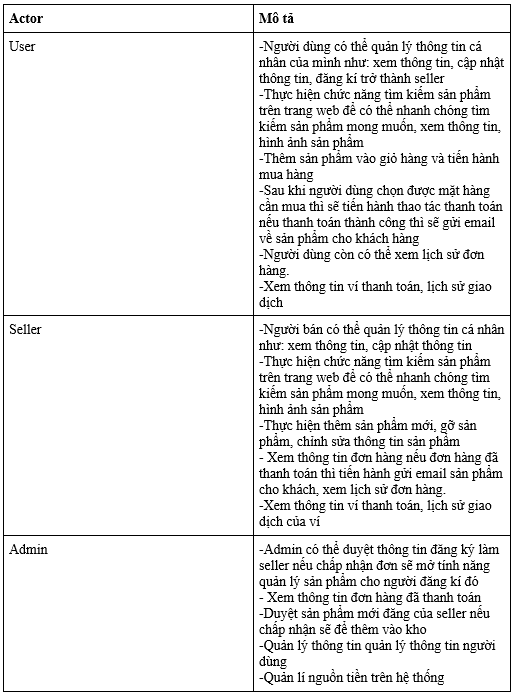
\includegraphics{anh3.png}
			
		\end{center}
		
		
	\end{figure}
\end{center}
\newpage
\subsection{Danh mục các Use-case của hệ thống}

\begin{center}
	\begin{figure}[htp]
		\begin{center}
			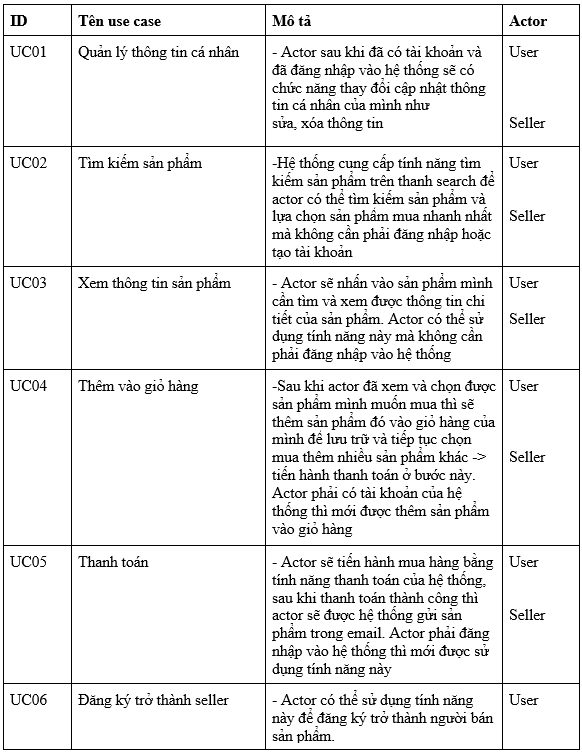
\includegraphics[scale=.930]{anh5.png}
		
		\end{center}
	
		
	\end{figure}
\end{center}
\newpage
\begin{center}
	\begin{figure}[htp]
		\begin{center}
		
			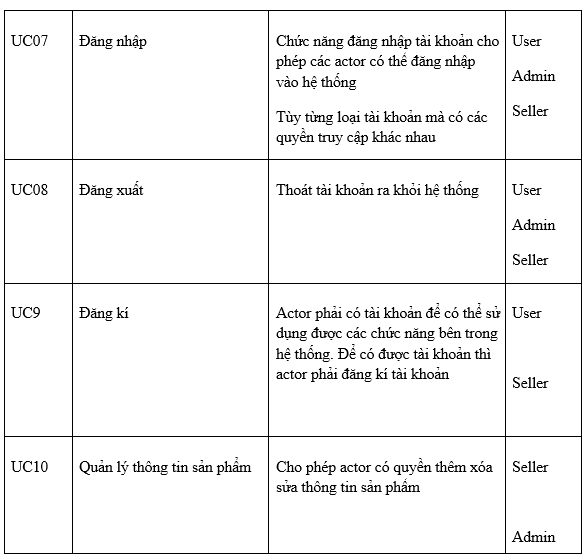
\includegraphics[scale=.930]{anh6.png}
			
		\end{center}
	
		
	\end{figure}
\end{center}
\newpage
\begin{center}
	\begin{figure}[htp]
		\begin{center}
			
			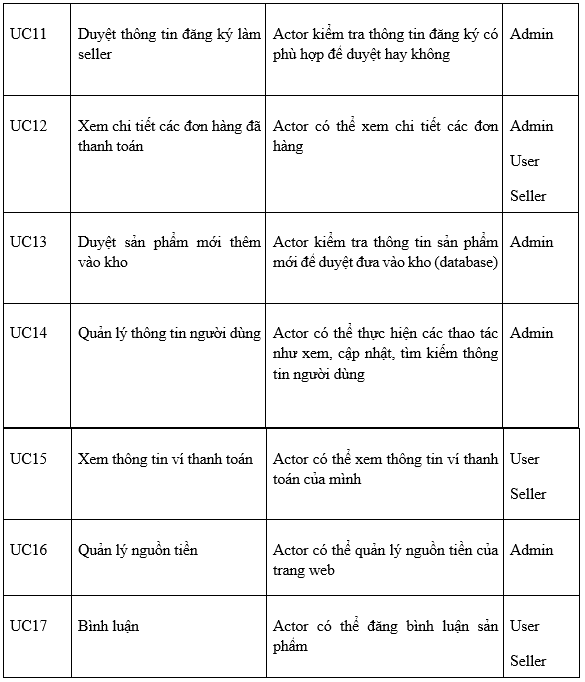
\includegraphics[scale=.930]{anh7.png}
			
		\end{center}
		
		
	\end{figure}
\end{center}
\newpage


\subsection{Lược đồ Use-case}


\begin{center}
	\begin{figure}[htp]
		\begin{center}
			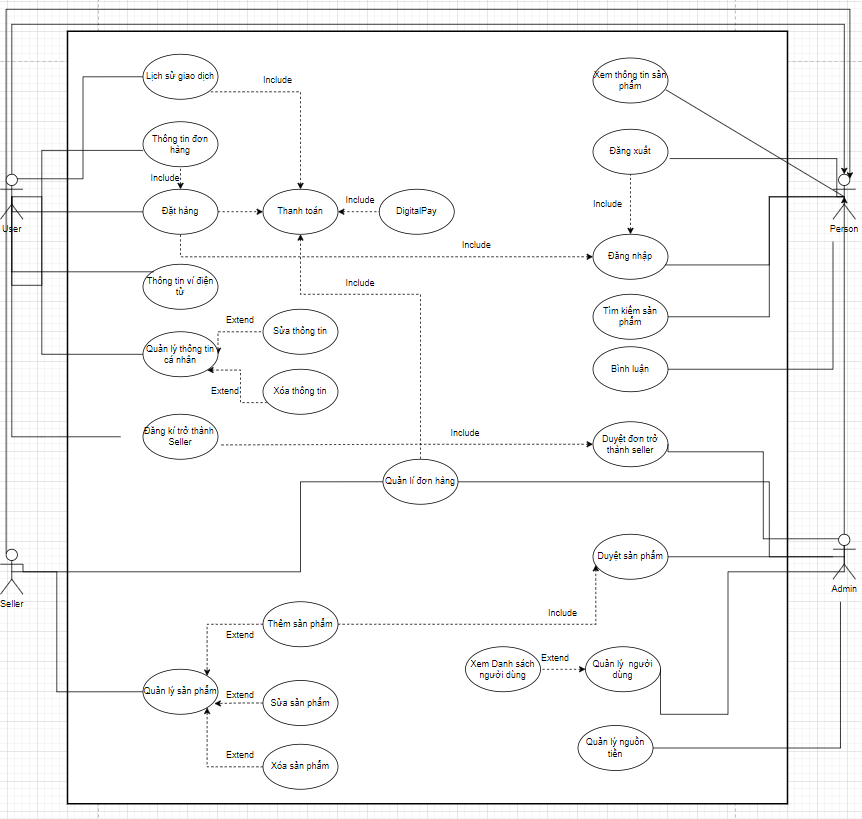
\includegraphics[scale=.750]{anh9.png}
		\end{center}
		\caption{Sơ đồ Use-case}
		
	\end{figure}
\end{center}



\subsection{Đặc tả Use-case}\newpage
{\large Đặc tả Use-case quản lý thông tin cá nhân
	
	\begin{center}
		\begin{figure}[htp]
			\begin{center}
				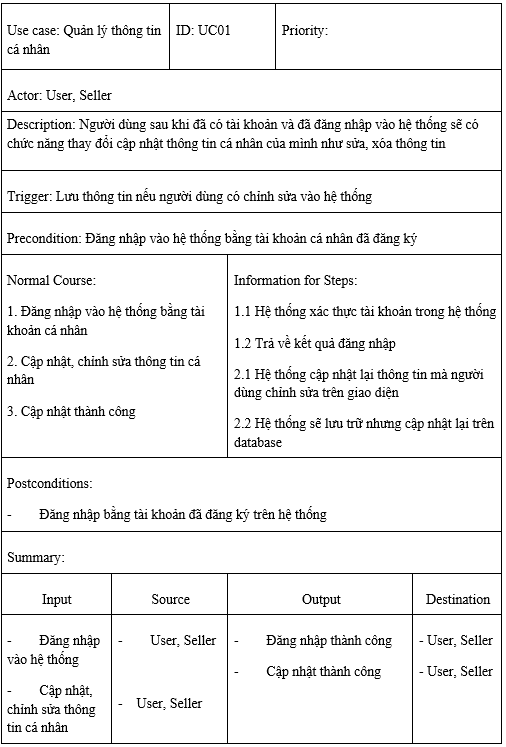
\includegraphics[scale=.870]{anh10.png}
			\end{center}
			\caption{Đặc tả Use-case quản lý sản phẩm}
			
		\end{figure}
	\end{center}
\newpage
{\large Đặc tả Use-case tìm kiếm sản phẩm
	
	\begin{center}
		\begin{figure}[htp]
			\begin{center}
				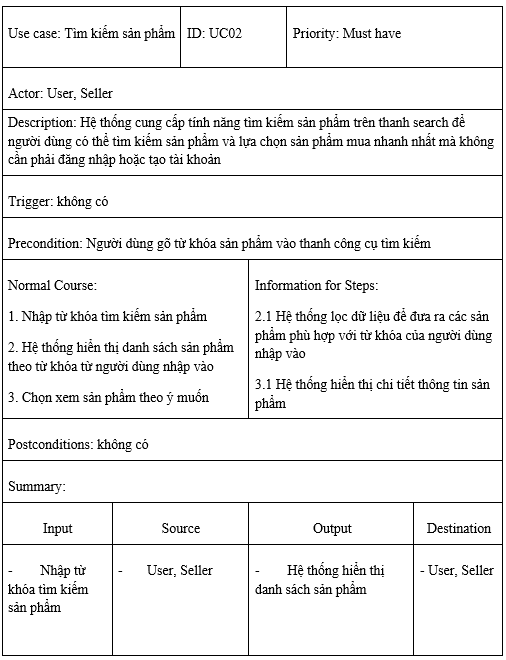
\includegraphics[scale=.950]{anh11.png}
			\end{center}
			\caption{Đặc tả Use-case tìm kiếm sản phẩm}
			
		\end{figure}
	\end{center}
\newpage
{\large Đặc tả Use-case xem thông tin sản phẩm
	
	\begin{center}
		\begin{figure}[htp]
			\begin{center}
				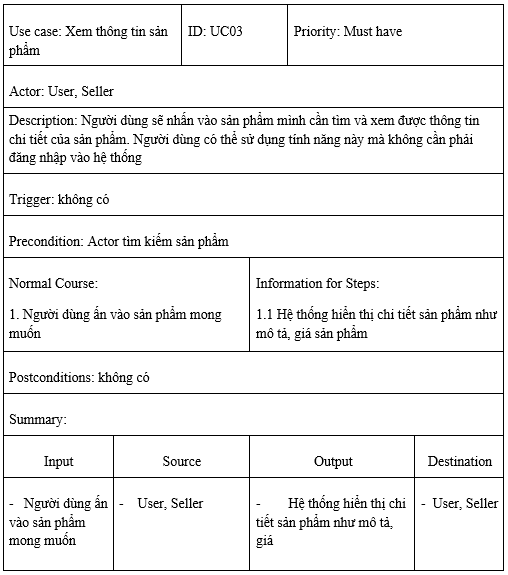
\includegraphics[scale=.950]{anh12.png}
			\end{center}
			\caption{Đặc tả Use-case xem thông tin sản phẩm}
			
		\end{figure}
	\end{center}
\newpage
{\large Đặc tả Use-case thêm vào giỏ hàng
	
	\begin{center}
		\begin{figure}[htp]
			\begin{center}
				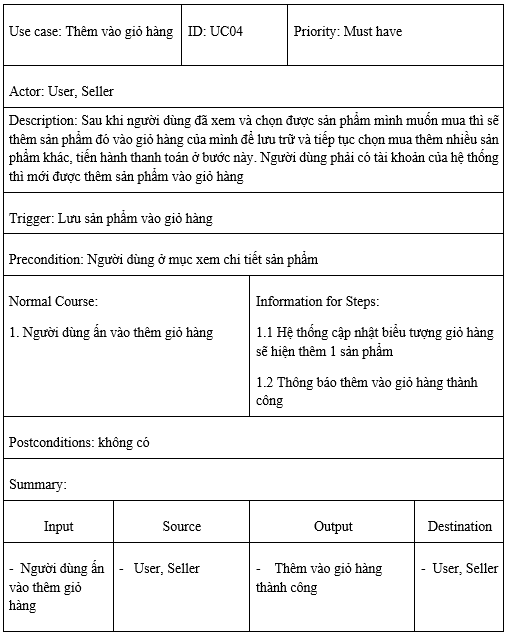
\includegraphics[scale=.945]{anh13.png}
			\end{center}
			\caption{Đặc tả Use-case thêm vào giỏ hàng}
			
		\end{figure}
	\end{center}
\newpage
{\large Đặc tả Use-case thanh toán
	\begin{center}
		\begin{figure}[htp]
			\begin{center}
				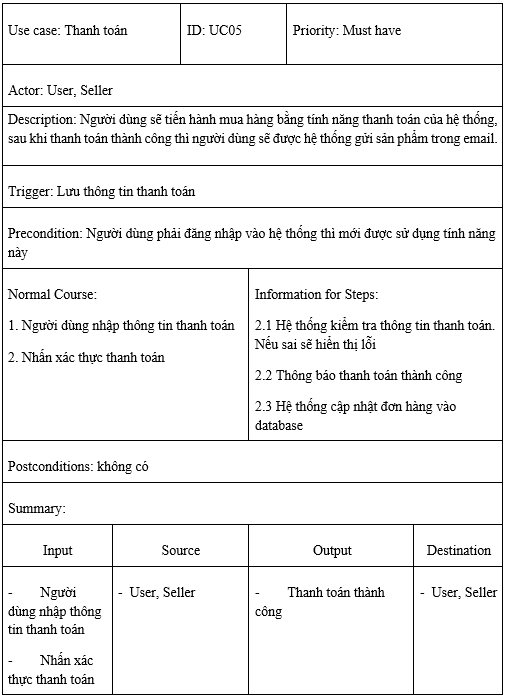
\includegraphics[scale=.895]{anh14.png}
			\end{center}
			\caption{Đặc tả Use-case thanh toán}
			
		\end{figure}
	\end{center}
\newpage

{\large Đặc tả Use-case đăng ký trở thành seller
	
	\begin{center}
		\begin{figure}[htp]
			\begin{center}
				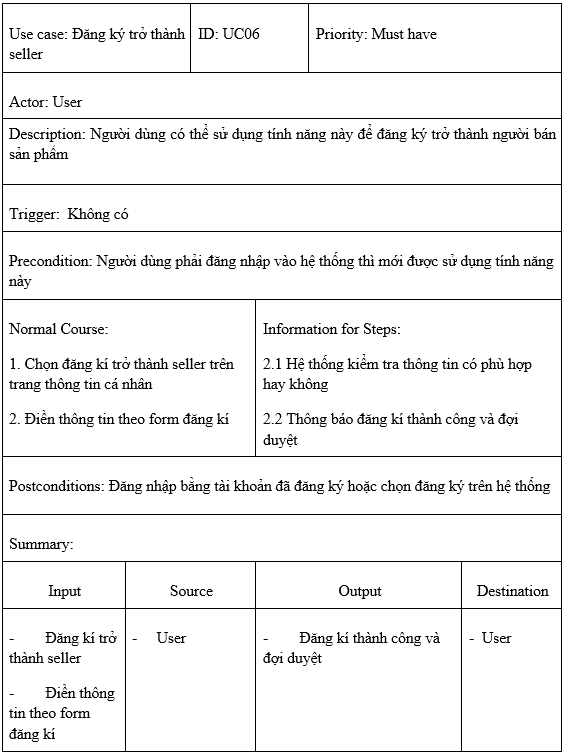
\includegraphics[scale=.850]{anh16.png}
			\end{center}
			\caption{Đặc tả Use-case đăng ký trở thành seller}
			
		\end{figure}
	\end{center}
\newpage
{\large Đặc tả Use-case đăng nhập
	
	\begin{center}
		\begin{figure}[htp]
			\begin{center}
				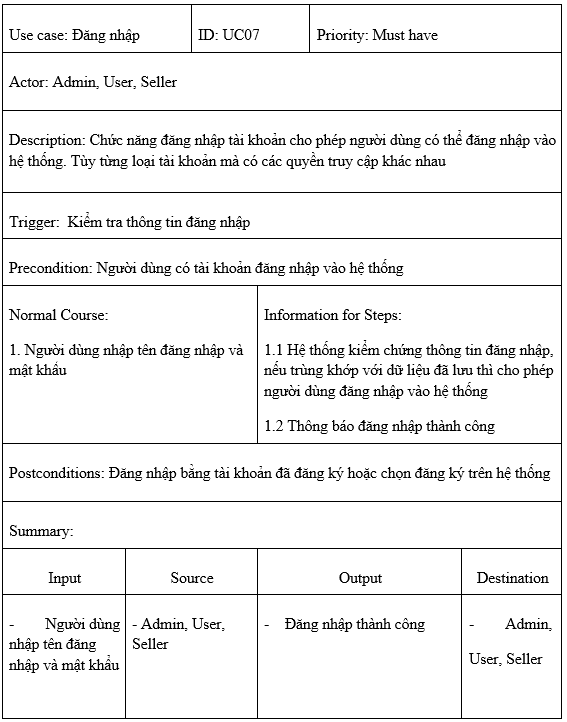
\includegraphics[scale=.865]{anh17.png}
			\end{center}
			\caption{Đặc tả Use-case đăng nhập}
			
		\end{figure}
	\end{center}
\newpage
{\large Đặc tả Use-case đăng xuất
	
	\begin{center}
		\begin{figure}[htp]
			\begin{center}
				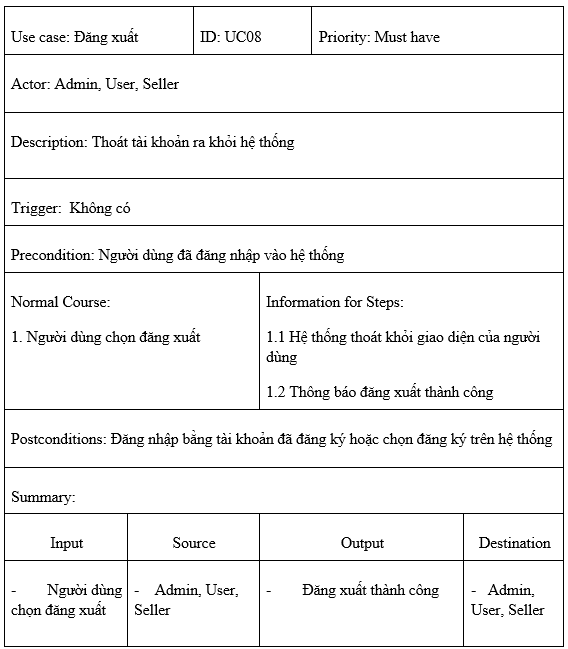
\includegraphics[scale=.890]{anh18.png}
			\end{center}
			\caption{Đặc tả Use-case đăng xuất}
			
		\end{figure}
	\end{center}
\newpage
{\large Đặc tả Use-case đăng kí
	
	\begin{center}
		\begin{figure}[htp]
			\begin{center}
				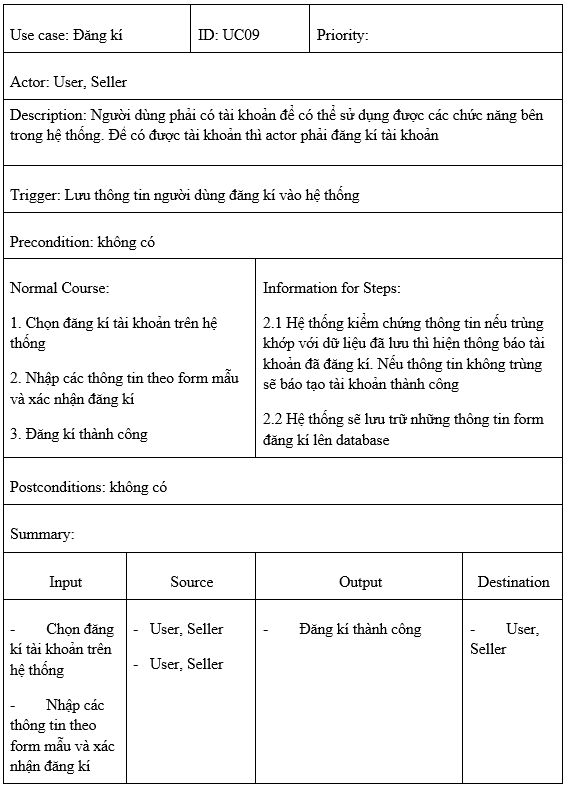
\includegraphics[scale=.830]{anh19.png}
			\end{center}
			\caption{Đặc tả Use-case đăng kí}
			
		\end{figure}
	\end{center}
\newpage
{\large Đặc tả Use-case quản lý thông tin sản phẩm
	
	\begin{center}
		\begin{figure}[htp]
			\begin{center}
				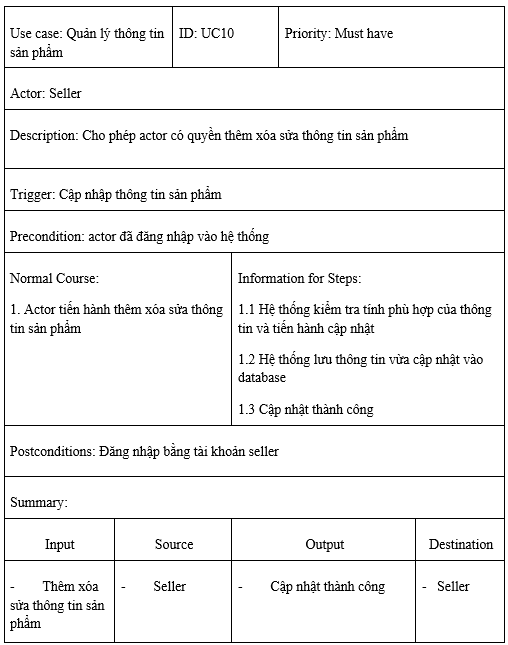
\includegraphics[scale=.900]{anh20.png}
			\end{center}
			\caption{Đặc tả Use-case quản lý thông tin sản phẩm}
			
		\end{figure}
	\end{center}
\newpage
{\large Đặc tả Use-case duyệt thông tin đăng kí làm seller
	
	\begin{center}
		\begin{figure}[htp]
			\begin{center}
				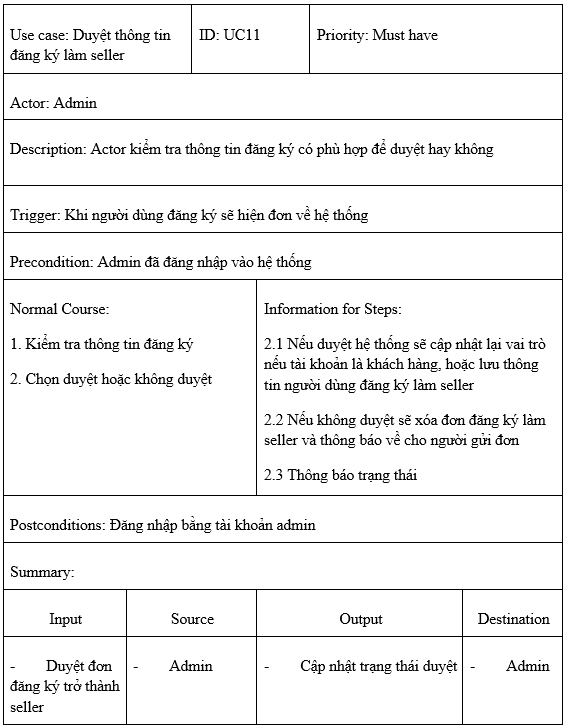
\includegraphics[scale=.900]{anh21.png}
			\end{center}
			\caption{Đặc tả Use-case duyệt thông tin đăng kí làm seller}
			
		\end{figure}
	\end{center}
\newpage
{\large Đặc tả Use-case xem chi tiết các đơn hàng đã thanh toán
	
	\begin{center}
		\begin{figure}[htp]
			\begin{center}
				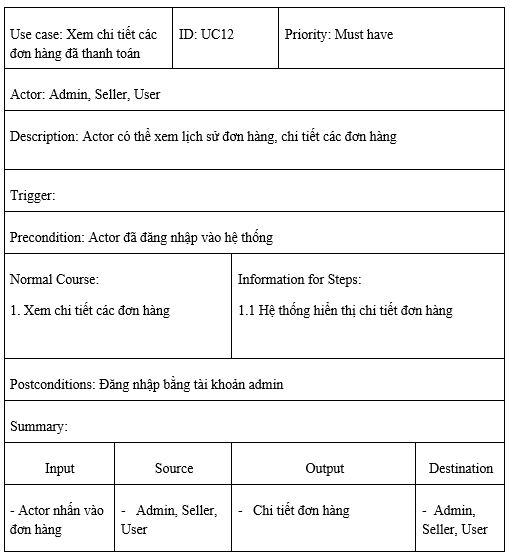
\includegraphics[scale=.950]{anh22.png}
			\end{center}
			\caption{Đặc tả Use-case xem chi tiết các đơn hàng đã thanh toán }
			
		\end{figure}
	\end{center}
\newpage
{\large Đặc tả Use-case duyệt sản phẩm mới thêm vào kho
	
	\begin{center}
		\begin{figure}[htp]
			\begin{center}
				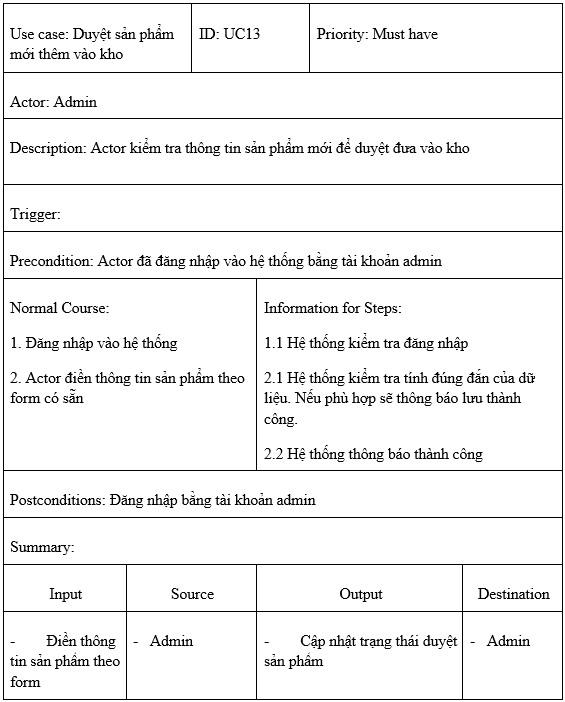
\includegraphics[scale=.950]{anh23.png}
			\end{center}
			\caption{Đặc tả Use-case duyệt sản phẩm mới thêm vào kho}
			
		\end{figure}
	\end{center}
\newpage
{\large Đặc tả Use-case quản lý thông tin người dùng
	
	\begin{center}
		\begin{figure}[htp]
			\begin{center}
				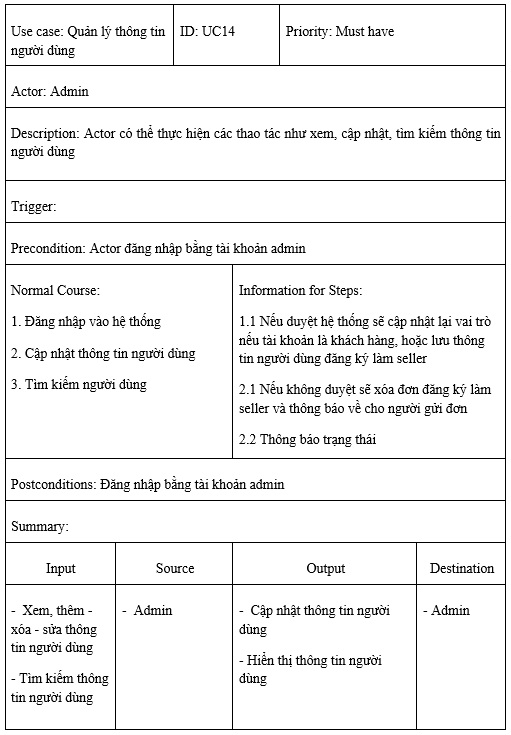
\includegraphics[scale=.810]{anh24.png}
			\end{center}
			\caption{Đặc tả Use-case quản lý thông tin người dùng}
			
		\end{figure}
	\end{center}
\newpage



\newpage
{\large Đặc tả Use-case xem thông tin ví thanh toán
	
	\begin{center}
		\begin{figure}[htp]
			\begin{center}
				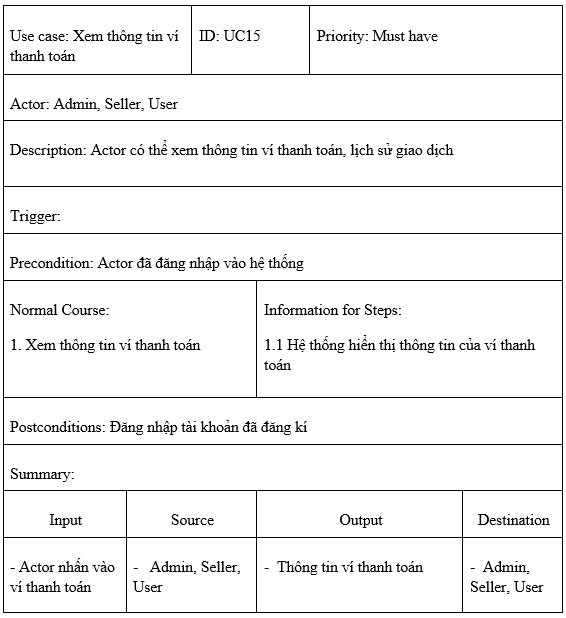
\includegraphics[scale=.930]{anh25.png}
			\end{center}
			\caption{Đặc tả Use-case xem thông tin ví thanh toán}
			
		\end{figure}
	\end{center}
	
	
\newpage
{\large Đặc tả Use-case quản lý nguồn tiền
	
	\begin{center}
		\begin{figure}[htp]
			\begin{center}
				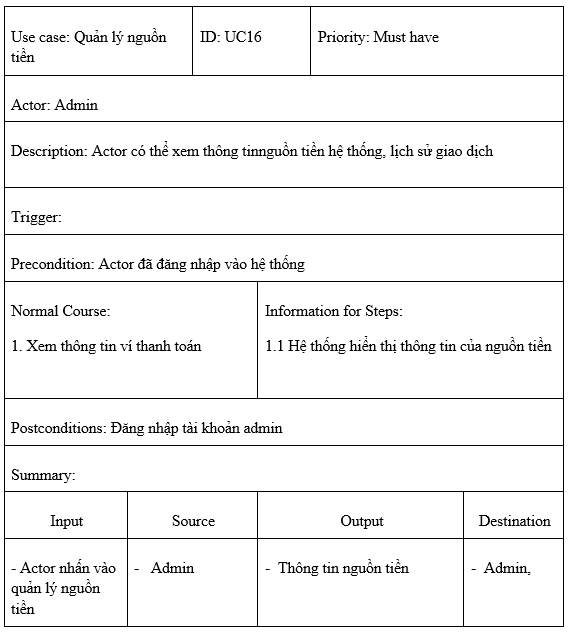
\includegraphics[scale=.930]{anh26.png}
			\end{center}
			\caption{Đặc tả Use-case quản lý nguồn tiền}
			
		\end{figure}
	\end{center}
	
\newpage
{\large Đặc tả Use-case bình luận
	
	\begin{center}
		\begin{figure}[htp]
			\begin{center}
				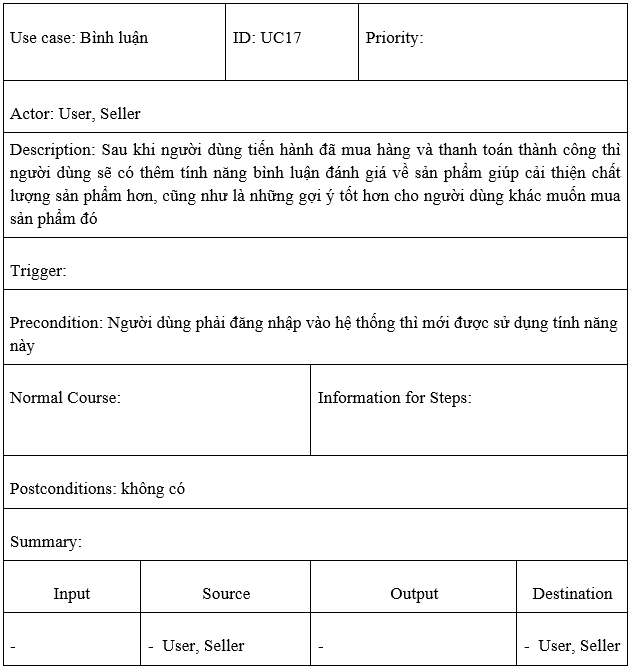
\includegraphics[scale=.930]{anh51.png}
			\end{center}
			\caption{Đặc tả Use-case bình luận}
			
		\end{figure}
	\end{center}
	
	\newpage
\subsection{Lược đồ ERD}
{\large Sơ đồ ERD

		\begin{center}
		\begin{figure}[htp]
			\begin{center}
				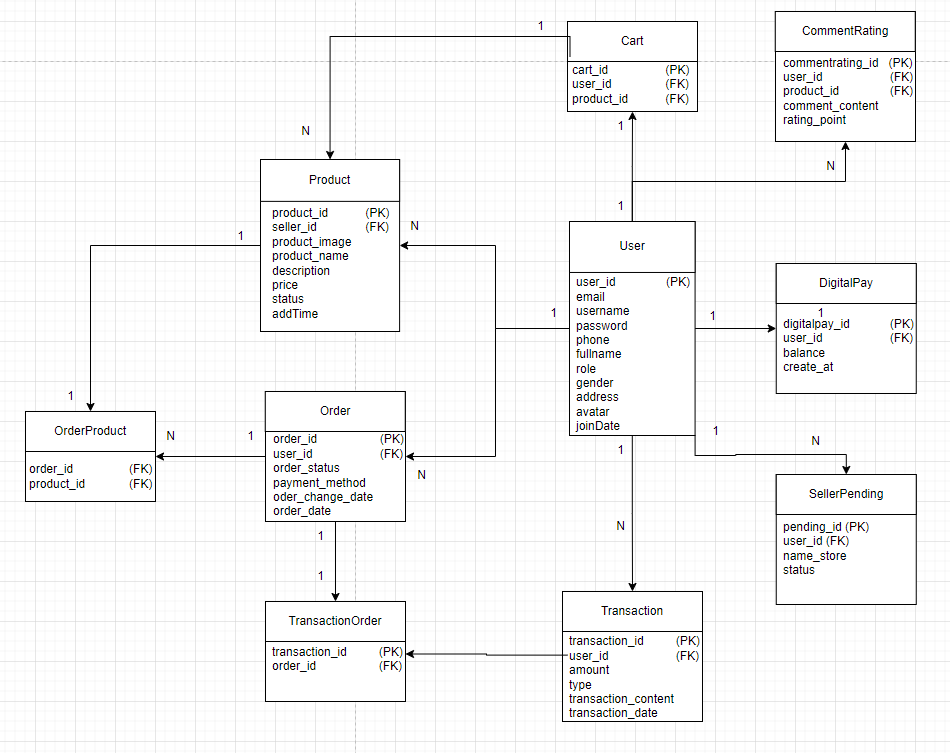
\includegraphics[scale=.700]{anh27.png}
			\end{center}
			\caption{Sơ đồ ERD}
			
		\end{figure}
	\end{center}
}


\newpage
{\large  Tổng quan sơ đồ ERD\\
	\indent Database hệ thống digital art thiết kế có 10 bảng Product chứa thông tin sản phẩm, Cart chứa thông tin giỏ hàng, CommentRating chứa thông tin bình luận, User chứa thông tin tài khoản người dùng, DigitalPay chứa thông tin ví điện tử,SellerPending chuwsathoong tin form đăng kí thành seller, Order chứa thông tin đơn hàng. Quan hệ giữa bảng User với các bảng Transaction, SellerPending, CommentRating, Product, Order là qua hệ mọt nhiều. Quan hệ giữa bảng User với các bảng Cart và DigitalPay là quan hệ một một. Quan hệ giữa bảng Cart và Product là quan hệ một nhiều, quan hệ giữa Procduct và OrderProduct là một một. Quan hệ giữa bảng Order với OrderProduct là một nhiều , quan hệ giữa bảng Order với TransactionOrder là một một.
	
	
}




\newpage
\section{HIỆN THỰC HỆ THỐNG}
\label{sec:Hiện thực hệ thống}
\subsection{Framework sử dụng }
{\large Nhóm chúng em sử dụng Node JS để làm backend và React JS để làm frontend để hiện thực sản phẩm: \\ 
	\indent Node JS\\
	\indent Node JS  là một nền tảng (Platform) phát triển độc lập được xây dựng trên V8 JavaScript Engine – trình thông dịch thực thi mã JavaScript giúp chúng ta có thể xây dựng được các ứng dụng web như các trang video clip, các forum và đặc biệt là trang mạng xã hội phạm vi hẹp một cách nhanh chóng và dễ dàng mở rộng.\\
\indent	Node JS có thể chạy trên nhiều nền tảng hệ điều hành khác nhau từ Window cho tới Linux, OS X nên đó cũng là một lợi thế. NodeJS cung cấp các thư viện phong phú ở dạng Javascript Module khác nhau giúp đơn giản hóa việc lập trình và giảm thời gian ở mức thấp nhất.\\
\indent Ý tưởng chính của Node JS là sử dụng non-blocking, hướng sự vào ra dữ liệu thông qua các tác vụ thời gian thực một cách nhanh chóng. Bởi vì, Node JS có khả năng mở rộng nhanh chóng, khả năng xử lý một số lượng lớn các kết nối đồng thời bằng thông lượng cao.\\

\indent	React JS\\
\indent React (React JS hay React.js) là 1 thư viện JavaScript mã nguồn mở được phát triển bởi đội ngũ kỹ sư đến từ Facebook; nó được giới thiệu vào năm 2011, cho đến nay là đã được hơn 10 năm. Nguyên lý xây dựng của React dựa trên components (component-based approach), có thể tái sử dụng và phù hợp với ứng dụng 1 trang (Single Page Application – SPA). React giúp lập trình viên xây dựng giao diện người dùng dựa trên JSX (môt cú pháp mở rộng của JavaScript), tạo ra các DOM ảo (virtual DOM) để tối ưu việc render 1 trang web.\\
\indent React JS sau khi ra đời đã cho thấy sự phù hợp của nó trong việc phát triển các ứng dụng Web với nhiều chức năng được tích hợp. Nó đã tạo thành 1 xu thế, 1 hình mẫu phát triển website với nhiều chức năng, khả năng tương tác đa dạng với người dùng. Hiện tại sau hơn 10 năm phát triển thì React vẫn đang chiếm vị trí số 1 trong các thư viện Front-end hiện tại.\\

	
}



\newpage

\subsection{Kiến trúc hệ thống }

{
	\large Cấu trúc hệ thống Digital Art có các phần :\\
- Phần chung:\\
+ Đăng nhập , đăng xuất, đăng ký tài khoản.\\
- User và seller có các phần:\\
+ Quản lý thông tin cá nhân.\\
+ Thêm/xóa vào giỏ hàng.\\
+ Tìm kiếm sản phẩm.\\
+ Xem thông tin sản phẩm.\\
+ Đăng ký trở thành seller.\\
+ Thanh toán \\
+ Xem chi tiết đơn hàng.\\
+ Ví điện tử.\\
+ Bình luận.\\
- Seller có phần riêng:\\
+ Thêm sản phẩm mới\\
+ Gỡ sản phẩm\\
+ Chỉnh sửa thông tin sản phẩm\\
- Admin có phần riêng:\\
+ Quản lý thông tin người dùng (user, seller)\\
+ Duyệt thông tin đăng ký làm seller.\\
+ Duyệt sản phẩm seller đăng lên.\\
+ Quản lý nguồn tiền .\\
	
}
\newpage
\subsection{Danh sách API }
{\large 
	\begin{center}
		\begin{figure}[htp]
			\begin{center}
				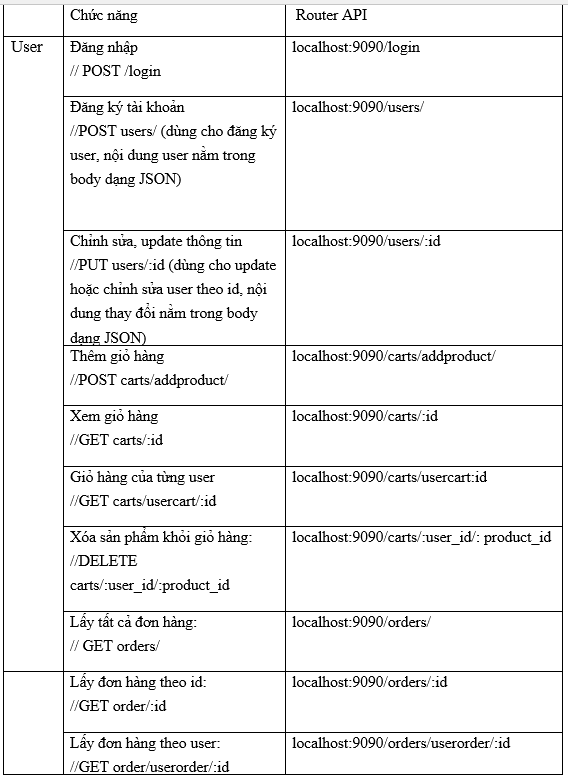
\includegraphics[scale=.900]{anh28.png}
			\end{center}
			
			
		\end{figure}
	\end{center}
}
\newpage
{\large 
	\begin{center}
		\begin{figure}[htp]
			\begin{center}
				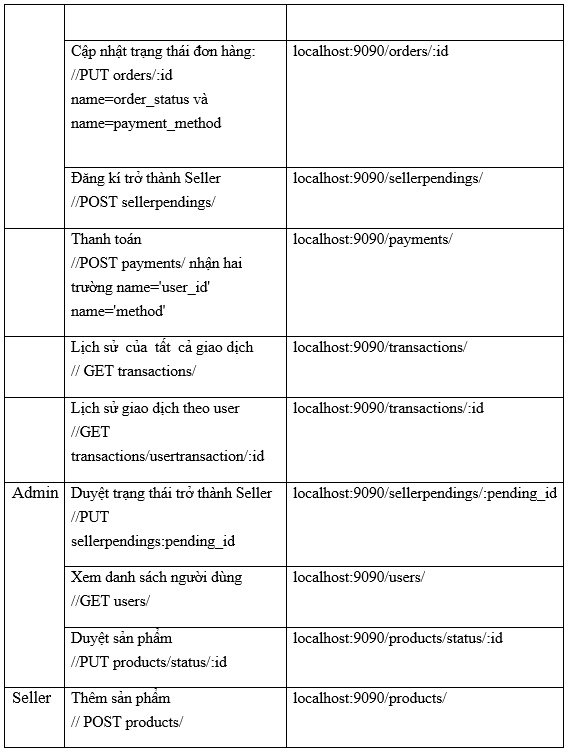
\includegraphics[scale=.900]{anh29.png}
			\end{center}
			
			
		\end{figure}
	\end{center}
}
\newpage
{\large 
	\begin{center}
		\begin{figure}[htp]
			\begin{center}
				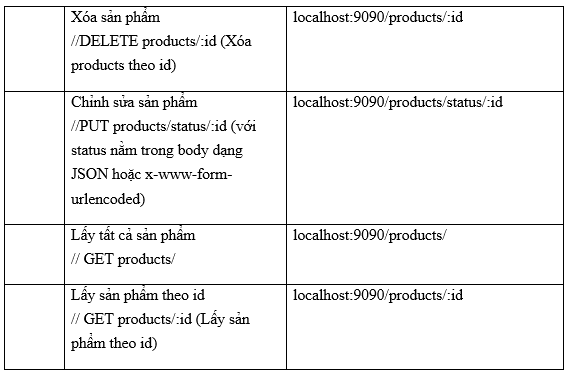
\includegraphics[scale=.900]{anh50.png}
			\end{center}
			
			
		\end{figure}
	\end{center}
}
\newpage
\section{DEMO}
\label{sec:Demo}
{\large Các tính năng của hệ thống Digital Art\\
	\indent	Trang chủ Digital Art\\
	\begin{center}
		\begin{figure}[htp]
			\begin{center}
				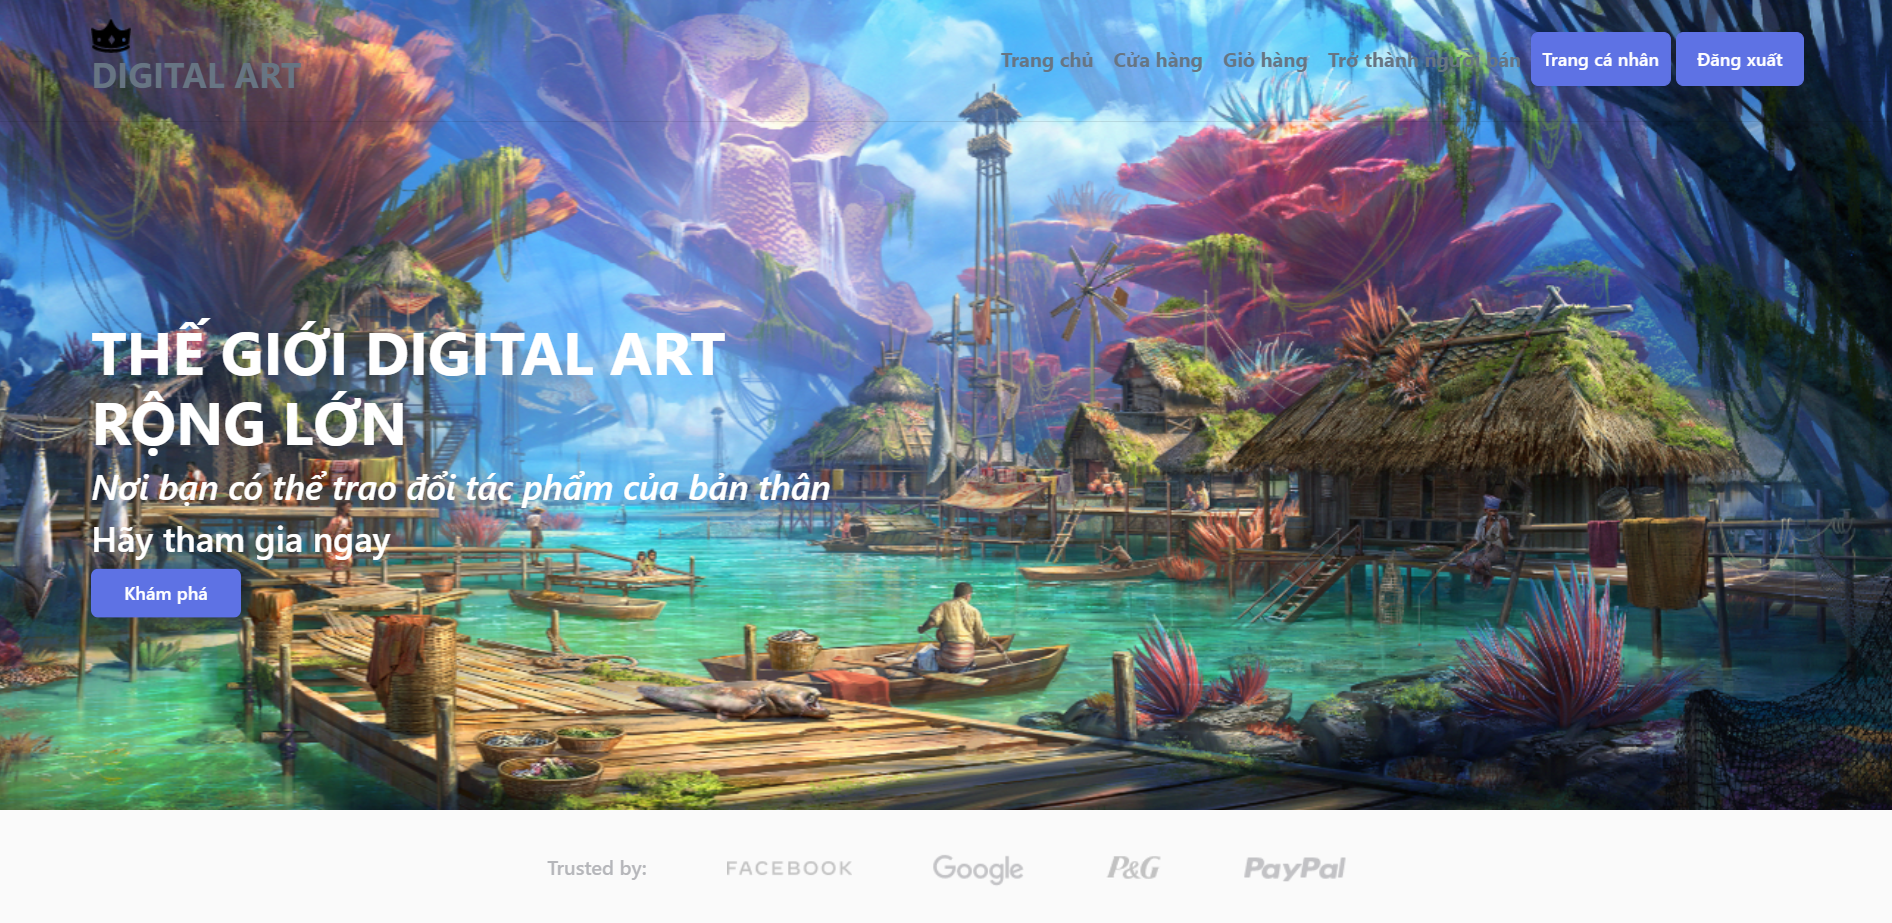
\includegraphics[scale=.350]{anh30.png}
			\end{center}
			\caption{Giao điện đăng nhập}
			
		\end{figure}
	\end{center}
}
\newpage
\indent	Đăng nhập\\
{\large
	Người dùng chọn vào mục đăng nhập trên trang chủ hệ thống sẽ chuyển tới trang đăng nhập hệ thống.}
	\begin{center}
		\begin{figure}[htp]
			\begin{center}
				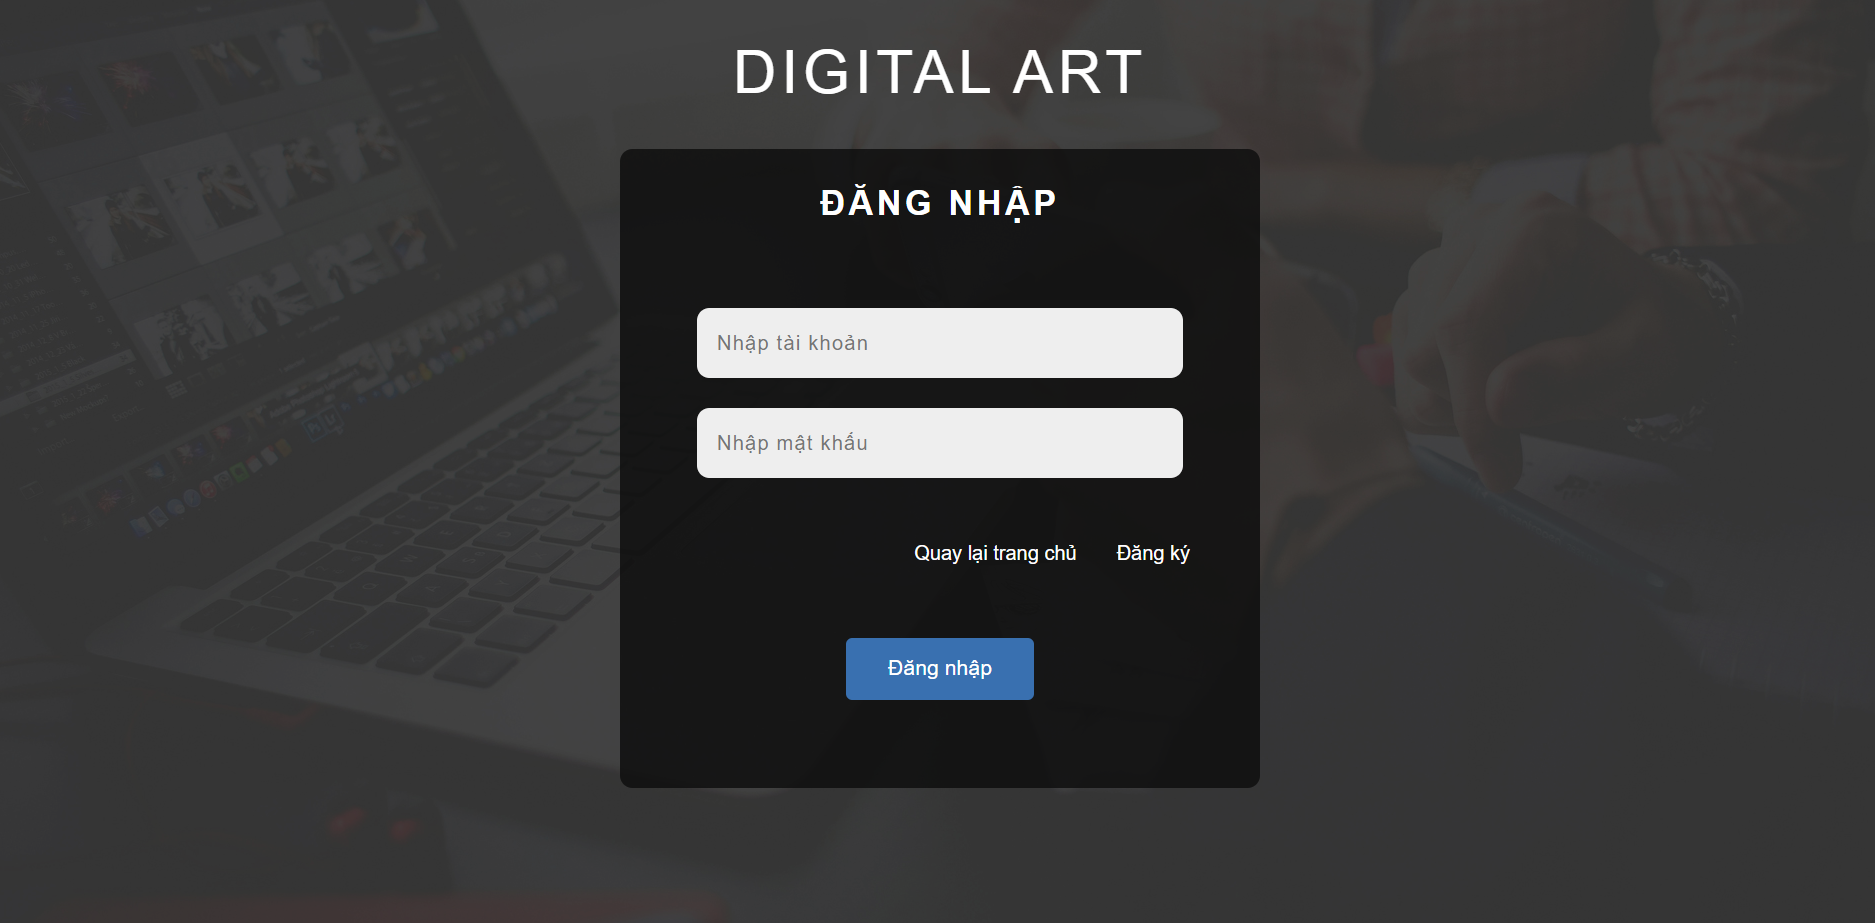
\includegraphics[scale=.350]{anh31.png}
			\end{center}
			\caption{Giao điện đăng nhập}
			
		\end{figure}
	\end{center}
}
\newpage
{\large 
	\indent	Đăng kí\\
	{\large
		Người dùng chọn vào mục đăng kí trên trang chủ hoặc trên đăng nhập hệ thống sẽ chuyển tới trang đăng ký tài khoản.}
	\begin{center}
		\begin{figure}[htp]
			\begin{center}
				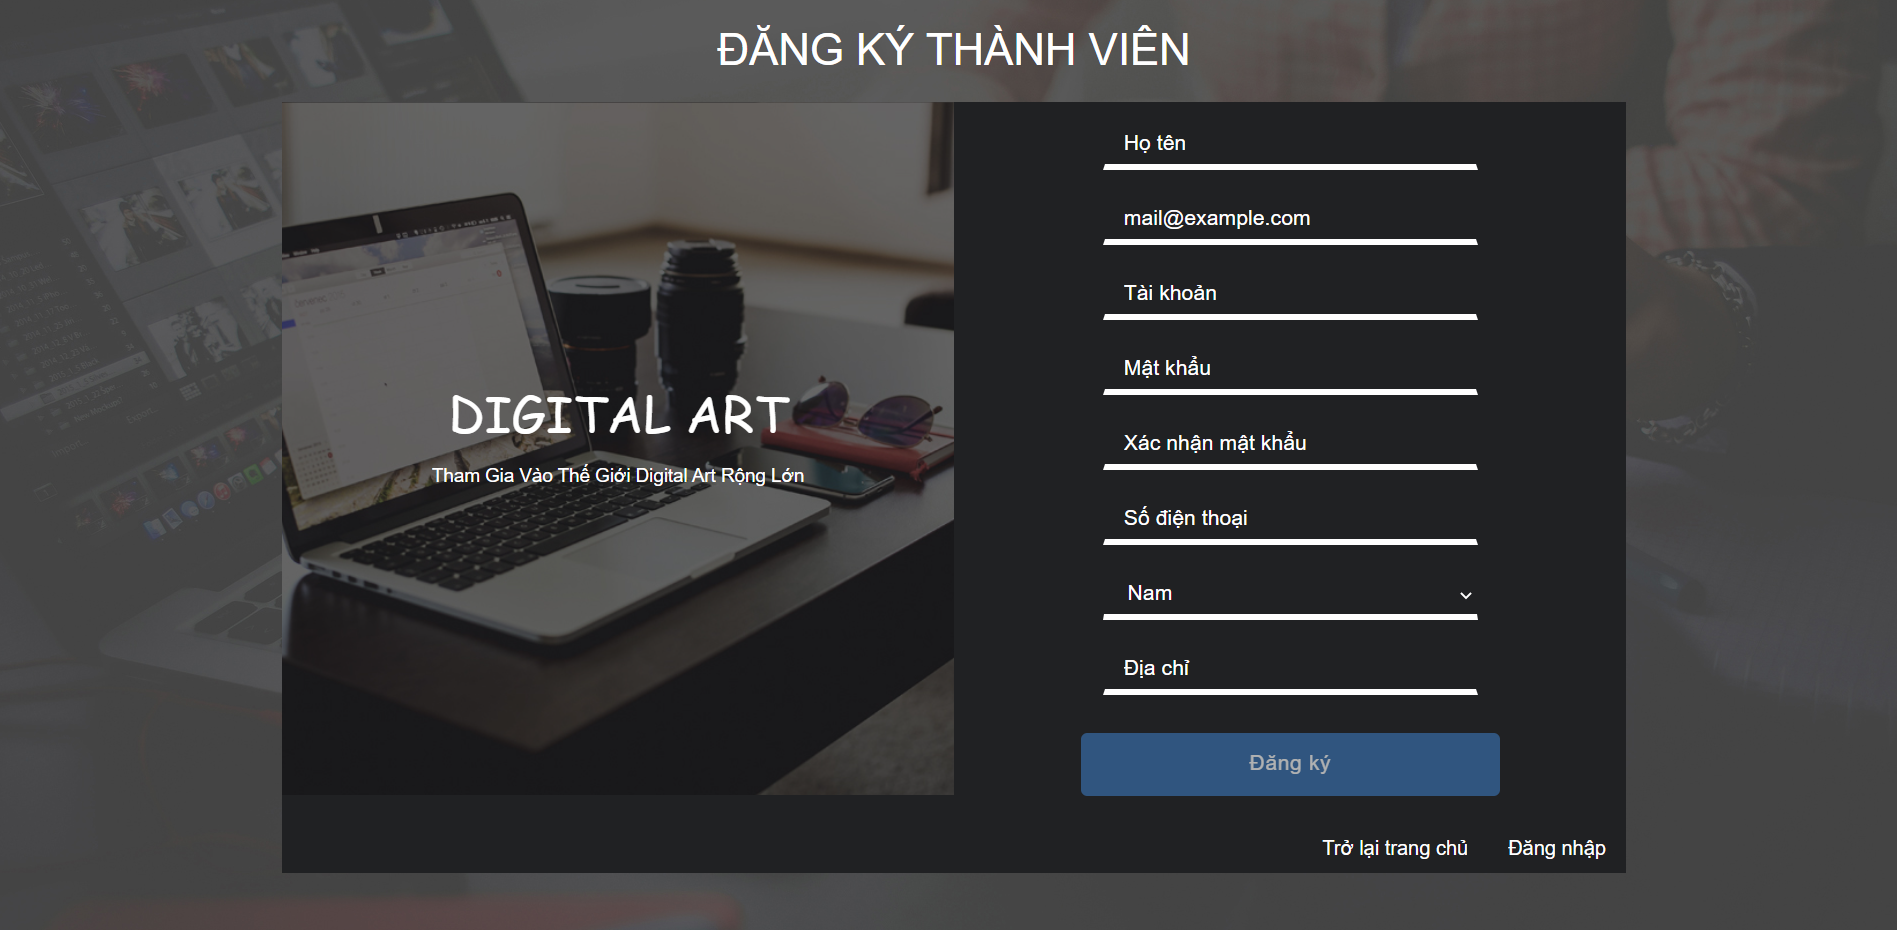
\includegraphics[scale=.350]{anh32.png}
			\end{center}
			\caption{Giao diện đăng kí}
			
		\end{figure}
	\end{center}
}
\newpage
{\large 
	\indent	Đăng ký trở thành seller\\
		{\large
		Người dùng chọn vào mục trở thành người bán trên trang chủ hệ thống sẽ chuyển tới trang đăng ký trở thành seller.}
	\begin{center}
		\begin{figure}[htp]
			\begin{center}
				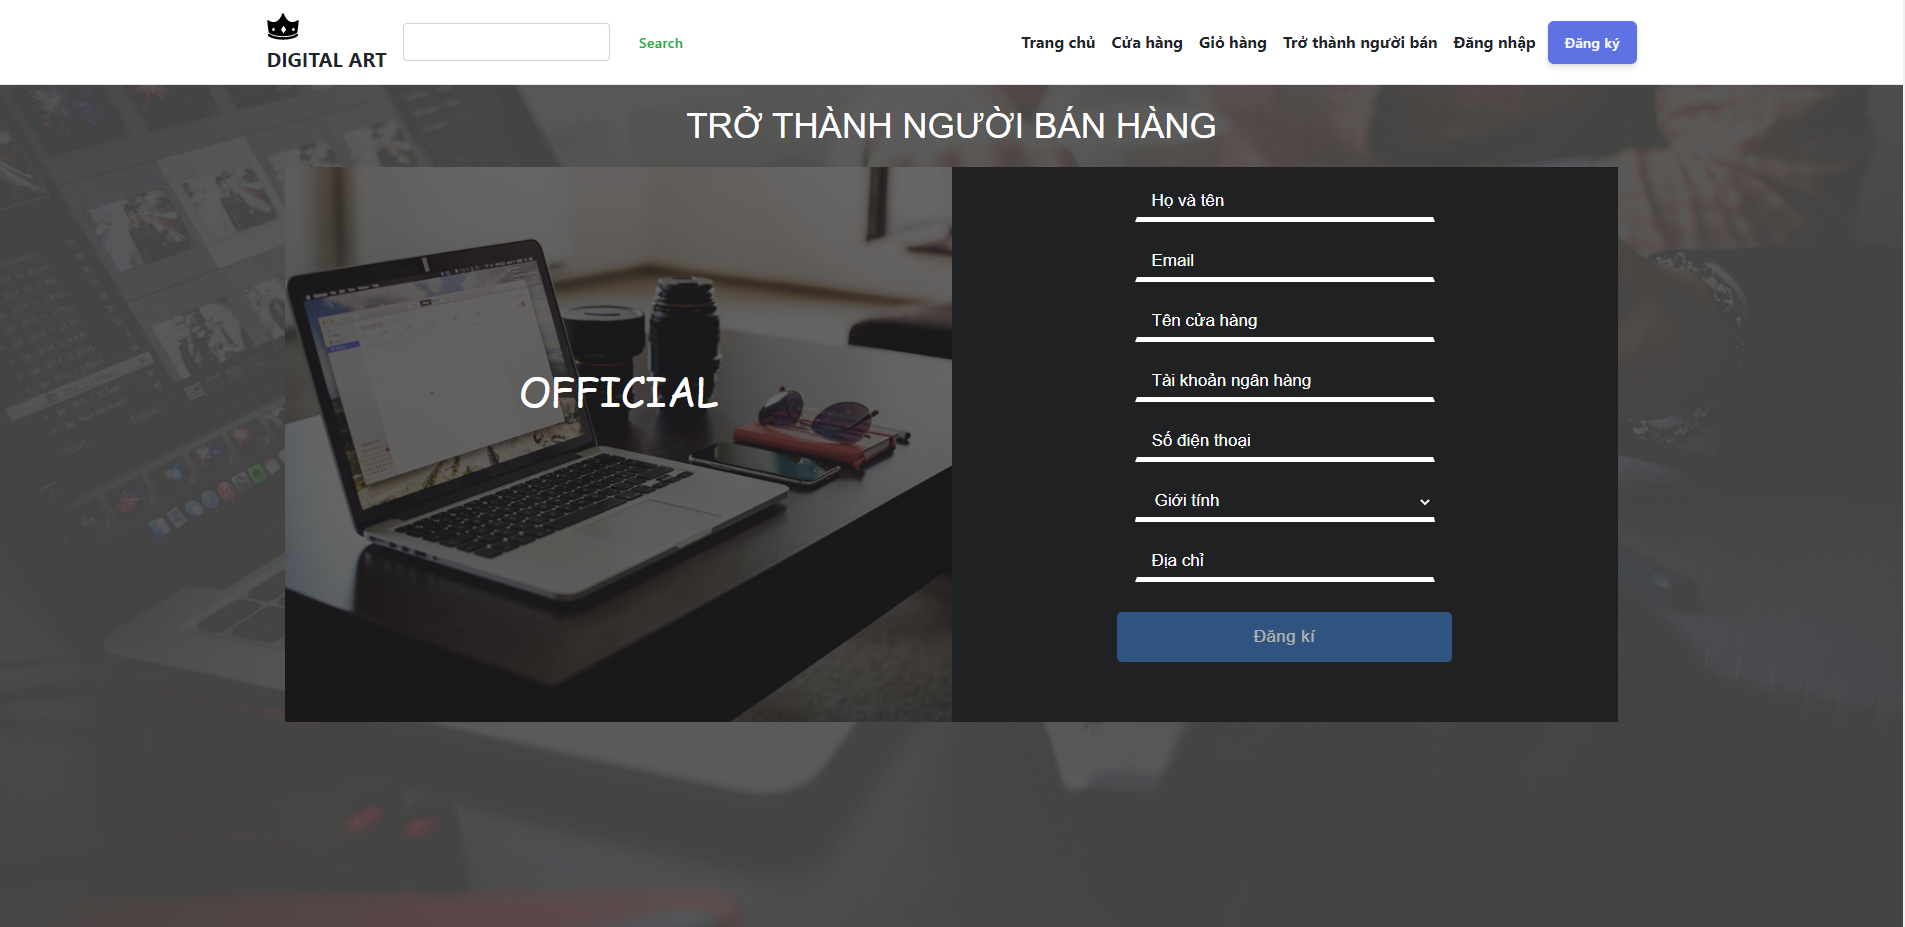
\includegraphics[scale=.350]{anh33.png}
			\end{center}
			\caption{Giao diện đăng ký trở thành seller}
			
		\end{figure}
	\end{center}
}

\newpage
{\large 
	\indent	Thêm/xóa vào giỏ hàng\\
	{\large
		Người dùng chọn vào mục giỏ hàng  trên trang chủ hoặc khi thêm sản phẩm vào giỏ hàng hệ thống sẽ chuyển tới trang giỏ hàng ở đây sẽ có tính năng thêm xóa giỏ hàng.}
	\begin{center}
		\begin{figure}[htp]
			\begin{center}
				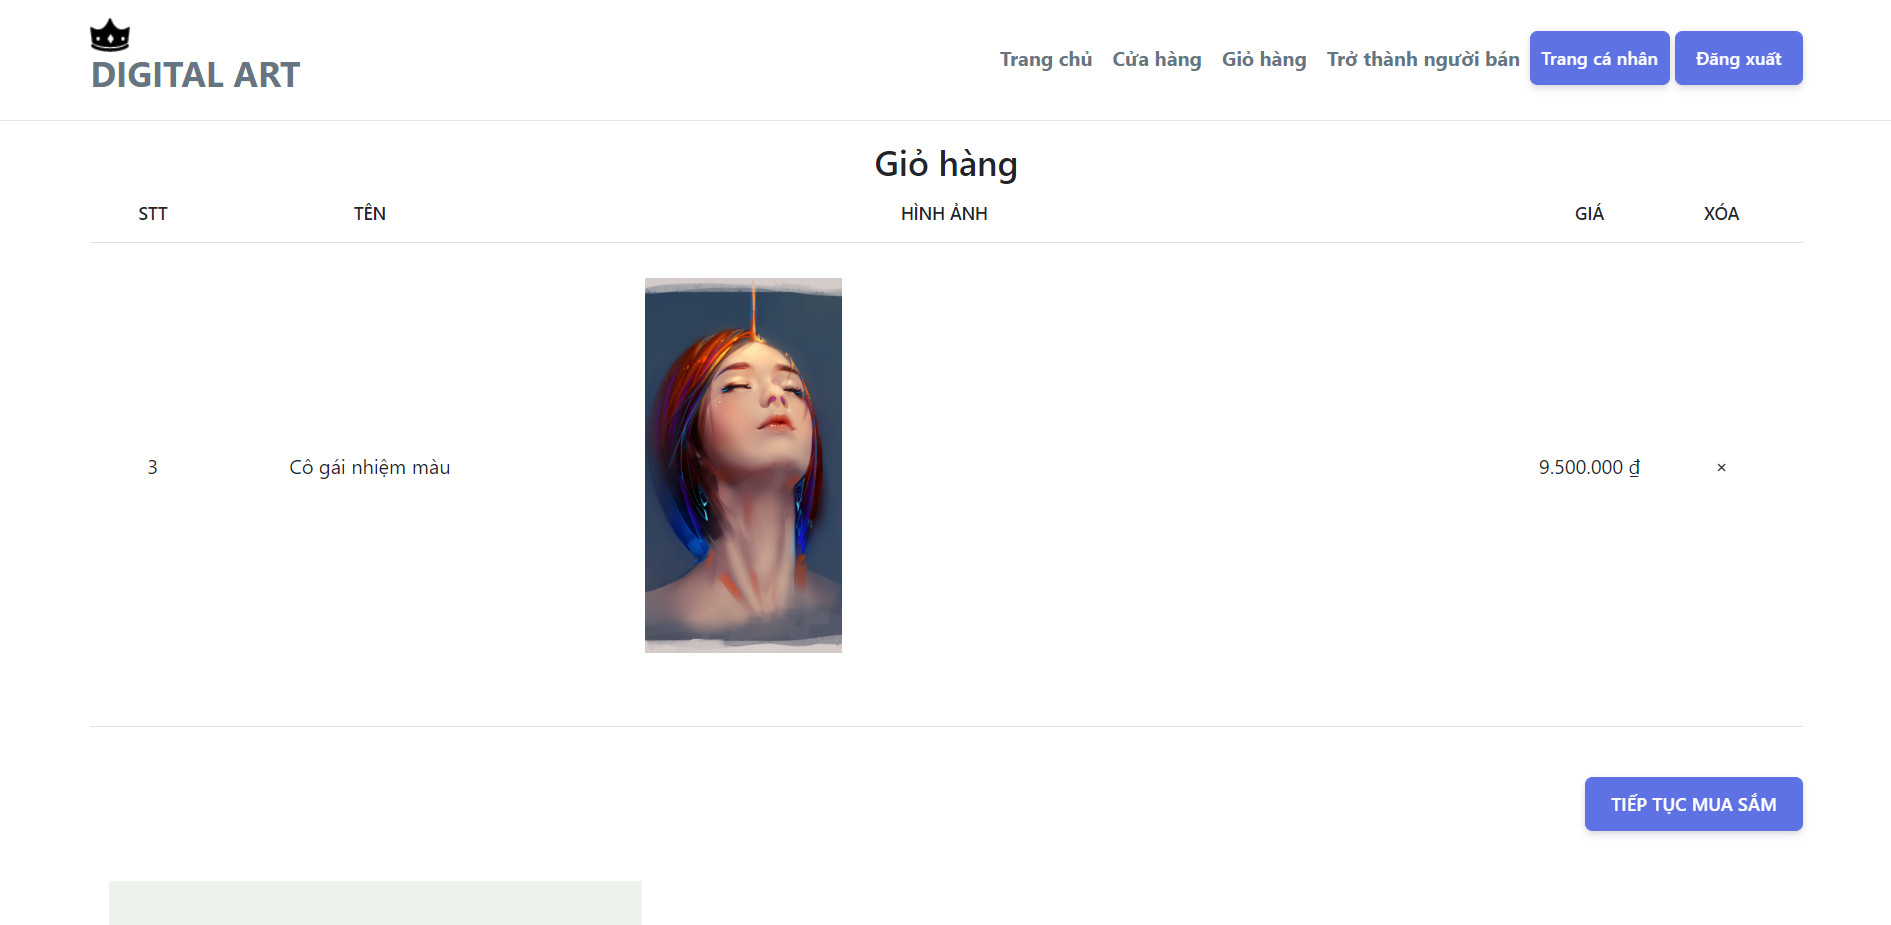
\includegraphics[scale=.250]{anh33.jpg}
			\end{center}
			\caption{Giao diện thêm/xóa vào giỏ hàng}
			
		\end{figure}
	\end{center}
}
\newpage

{\large 
	\indent	Xem thông tin sản phẩm\\
		{\large
		Người dùng chọn vào một sản phẩm hệ thống sẽ chuyển tới trang thông tin chi tiết của sản phẩm đó.}
	\begin{center}
		\begin{figure}[htp]
			\begin{center}
				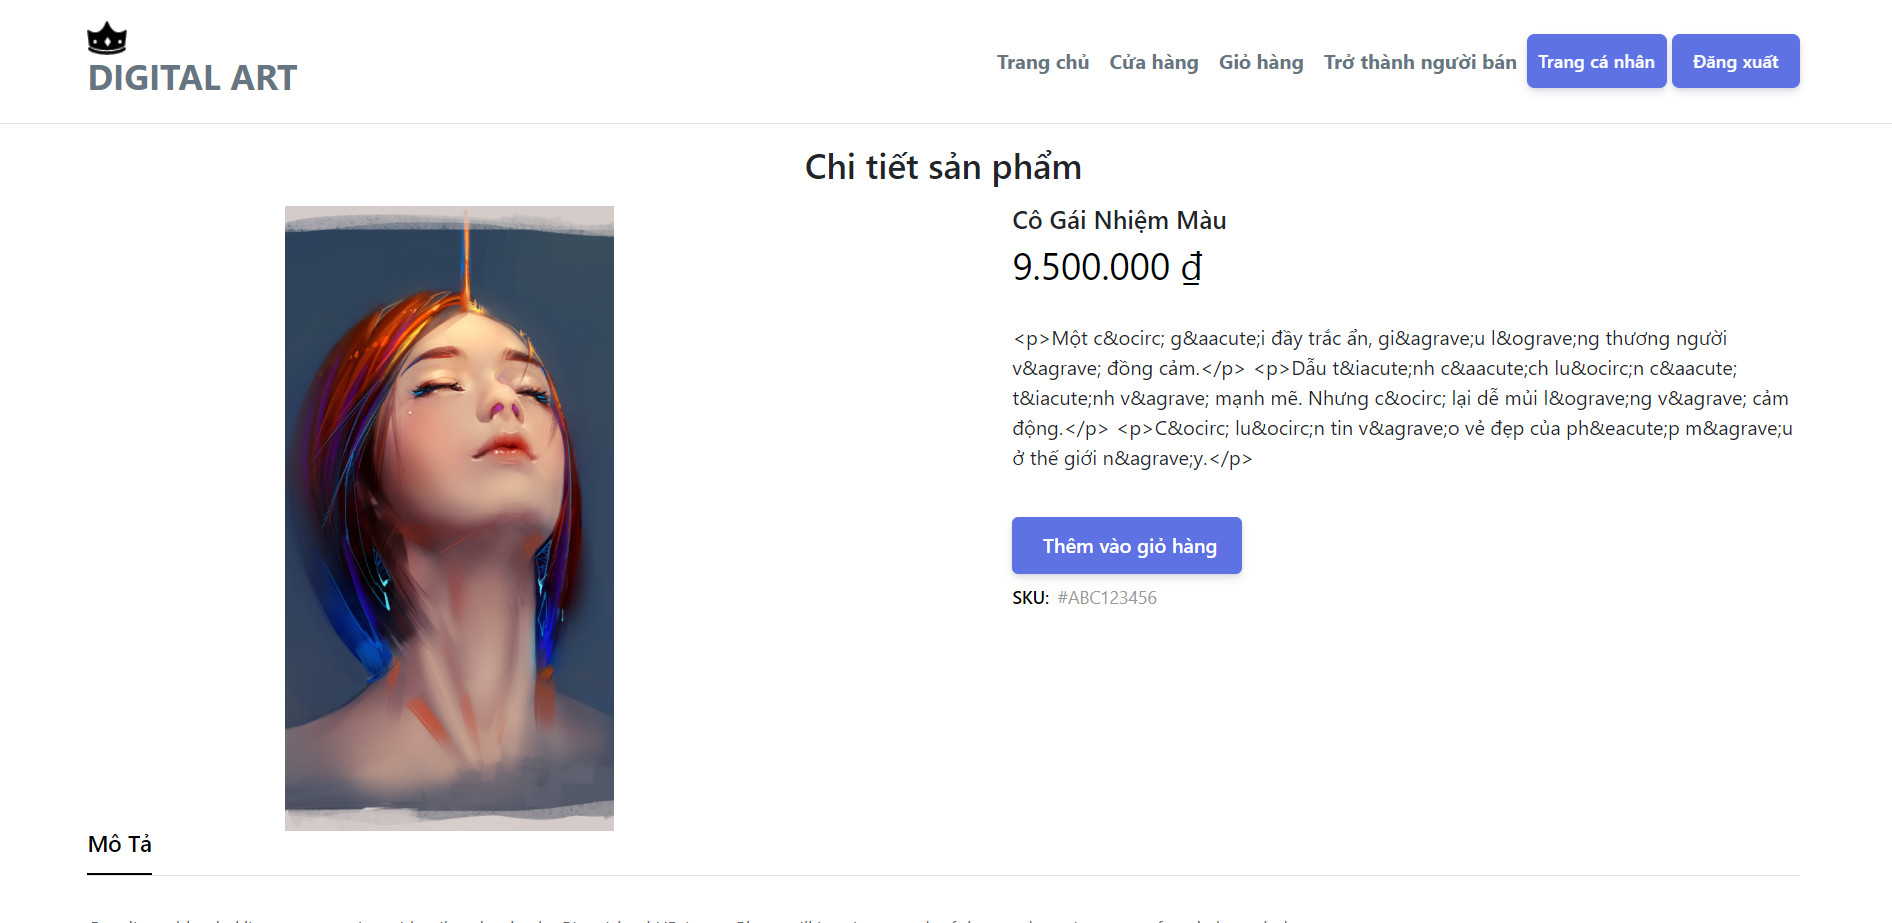
\includegraphics[scale=.250]{anh34.jpg}
			\end{center}
			\caption{Giao diện xem thông tin sản phẩm}
			
		\end{figure}
	\end{center}
}
\newpage
{\large 
	\indent	Thanh toán\\
	{\large
		Người dùng thêm sản phẩm vào giỏ hàng và ấn thanh toán  hệ thống sẽ chuyển tới trang thanh toán.}
	\begin{center}
		\begin{figure}[htp]
			\begin{center}
				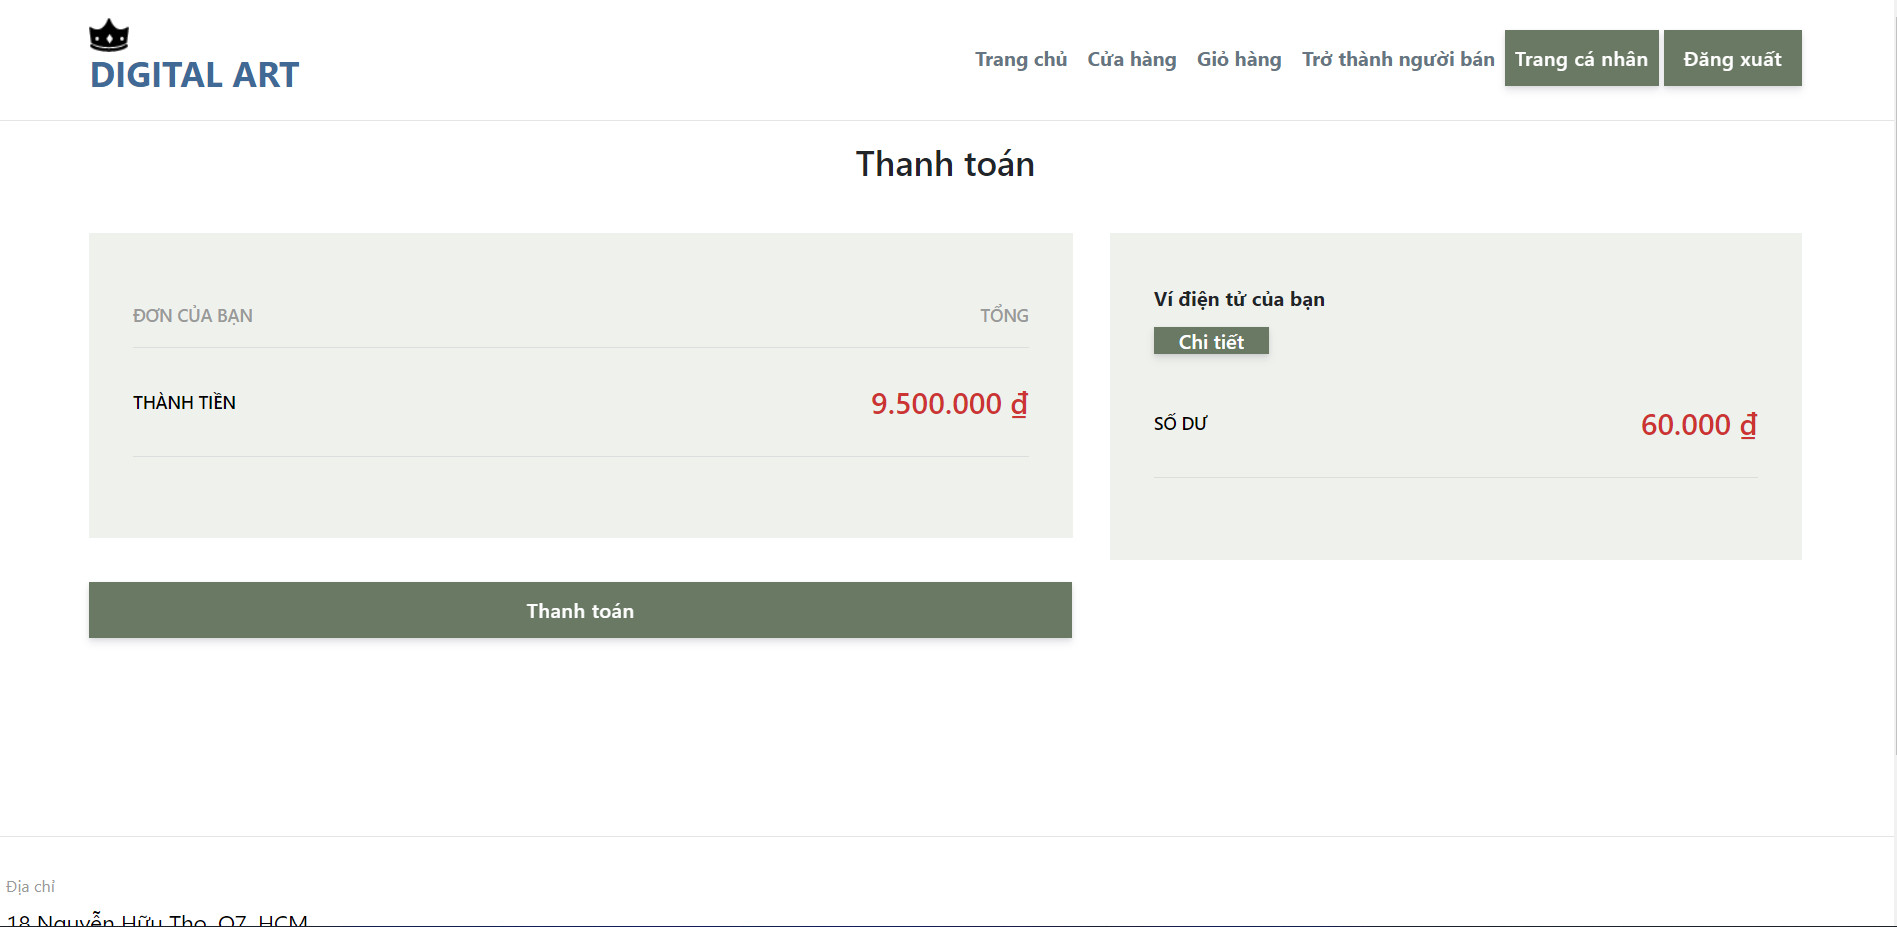
\includegraphics[scale=.250]{anh35.jpg}
			\end{center}
			\caption{Giao diện thanh toán}
			
		\end{figure}
	\end{center}
}
\newpage
{\large 
	\indent	Quản lý thông tin cá nhân\\
		{\large
		Người dùng ấn vào phần trang cá nhân trên trang chủ hệ thống sẽ chuyển tới trang thông tin cá nhân.}
	\begin{center}
		\begin{figure}[htp]
			\begin{center}
				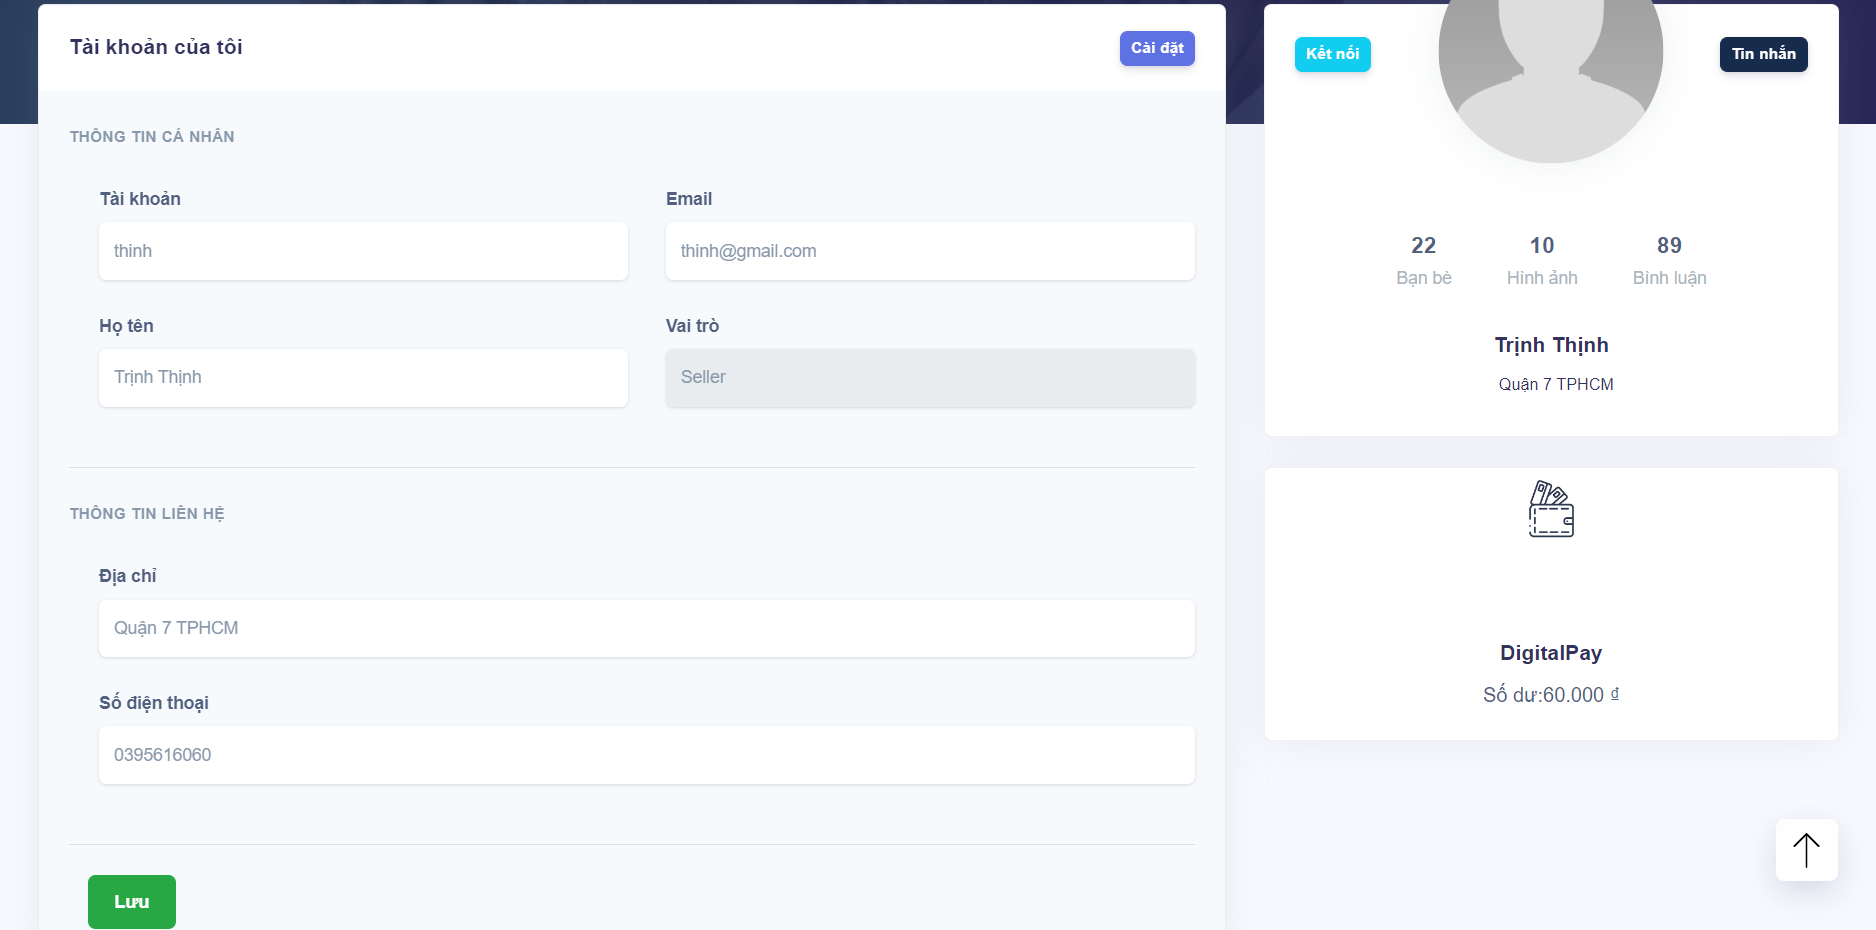
\includegraphics[scale=.350]{anh36.png}
			\end{center}
			\caption{Giao điện quản lý thông tin cá nhân}
			
		\end{figure}
	\end{center}
}


\newpage
{\large  
	\indent Thông tin ví điện tử người dùng\\
		{\large
		Người dùng ấn vào phần trang cá nhân trên trang chủ hệ thống sẽ chuyển tới trang thông tin cá nhân sau đó người dùng ấn vào thông tin ví  hệ thống sẽ chuyển tới trang thông tin ví điện tử của người dùng.}
	\begin{center}
		\begin{figure}[htp]
			\begin{center}
				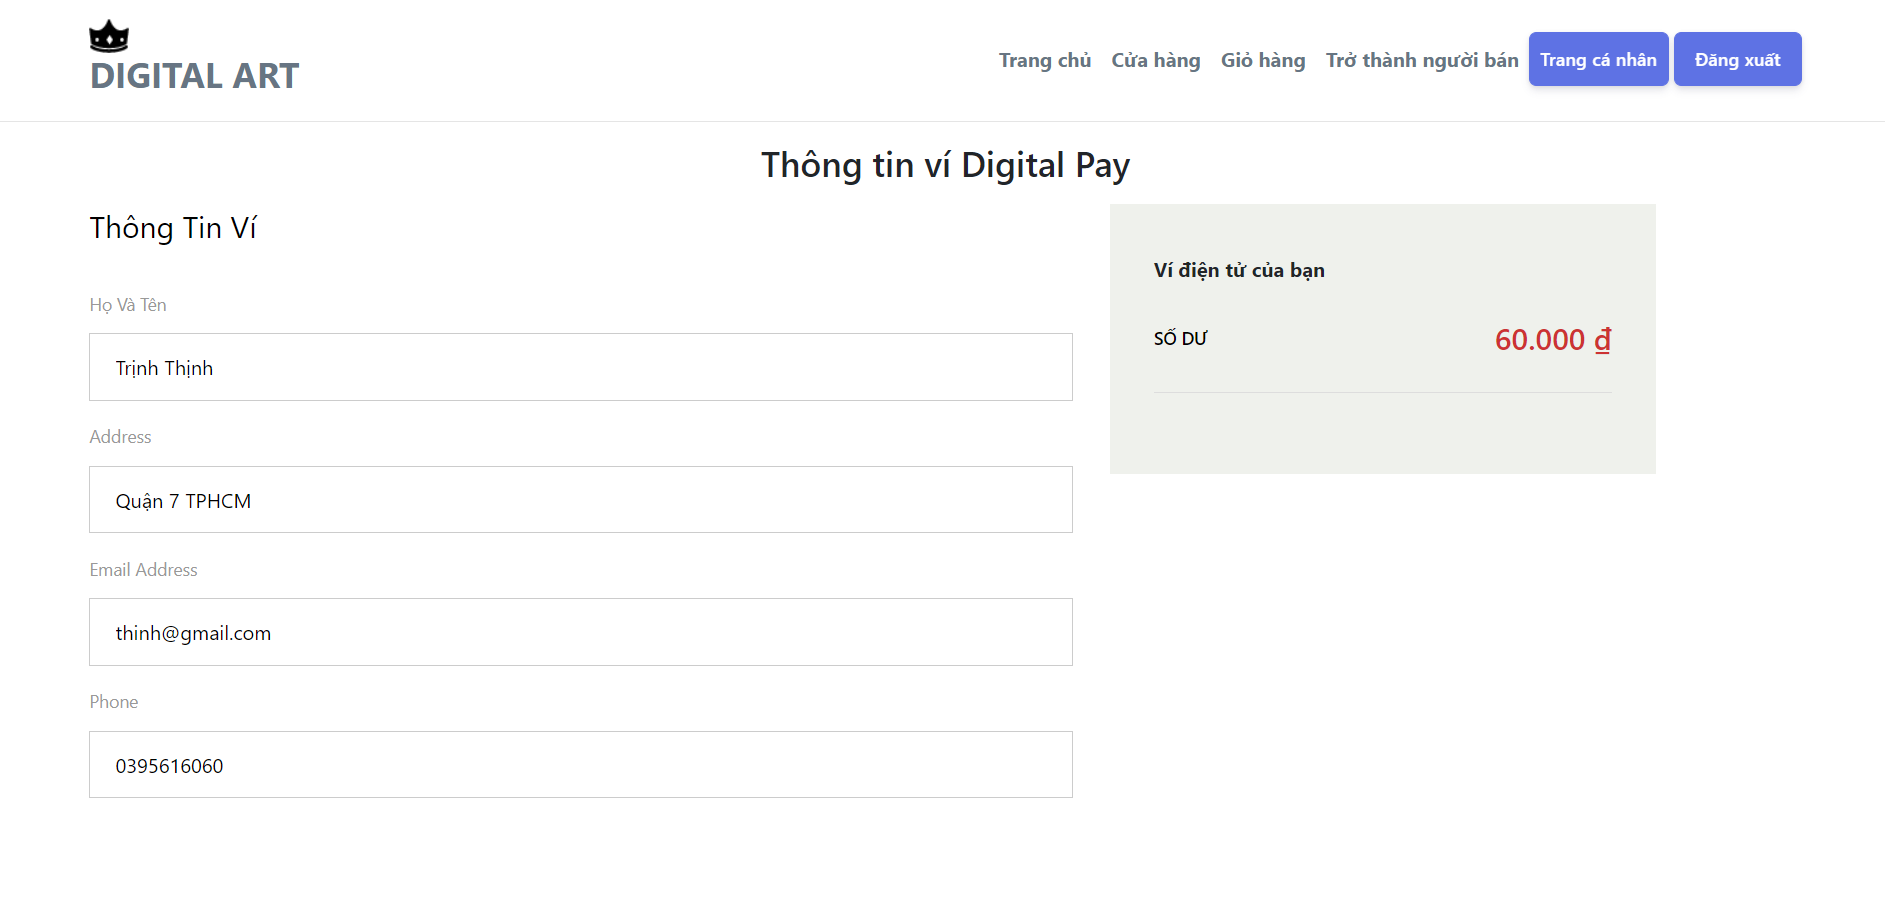
\includegraphics[scale=.400]{anh38.png}
			\end{center}
			\caption{Giao diện thông tin ví điện tử người dùng}
			
		\end{figure}
	\end{center}
}

\newpage
{\large  
	\indent Lịch sử đơn đặt hàng\\
	{\large
		Người dùng ấn vào phần thông tin cá nhân trên trang chủ hệ thống sẽ chuyển tới trang thông tin cá nhân sau đó người dùng ấn vào phần ví điện tử hệ thống sẽ chuyển tới trang thông tin ví điện tử của người dùng.}
	\begin{center}
		\begin{figure}[htp]
			\begin{center}
				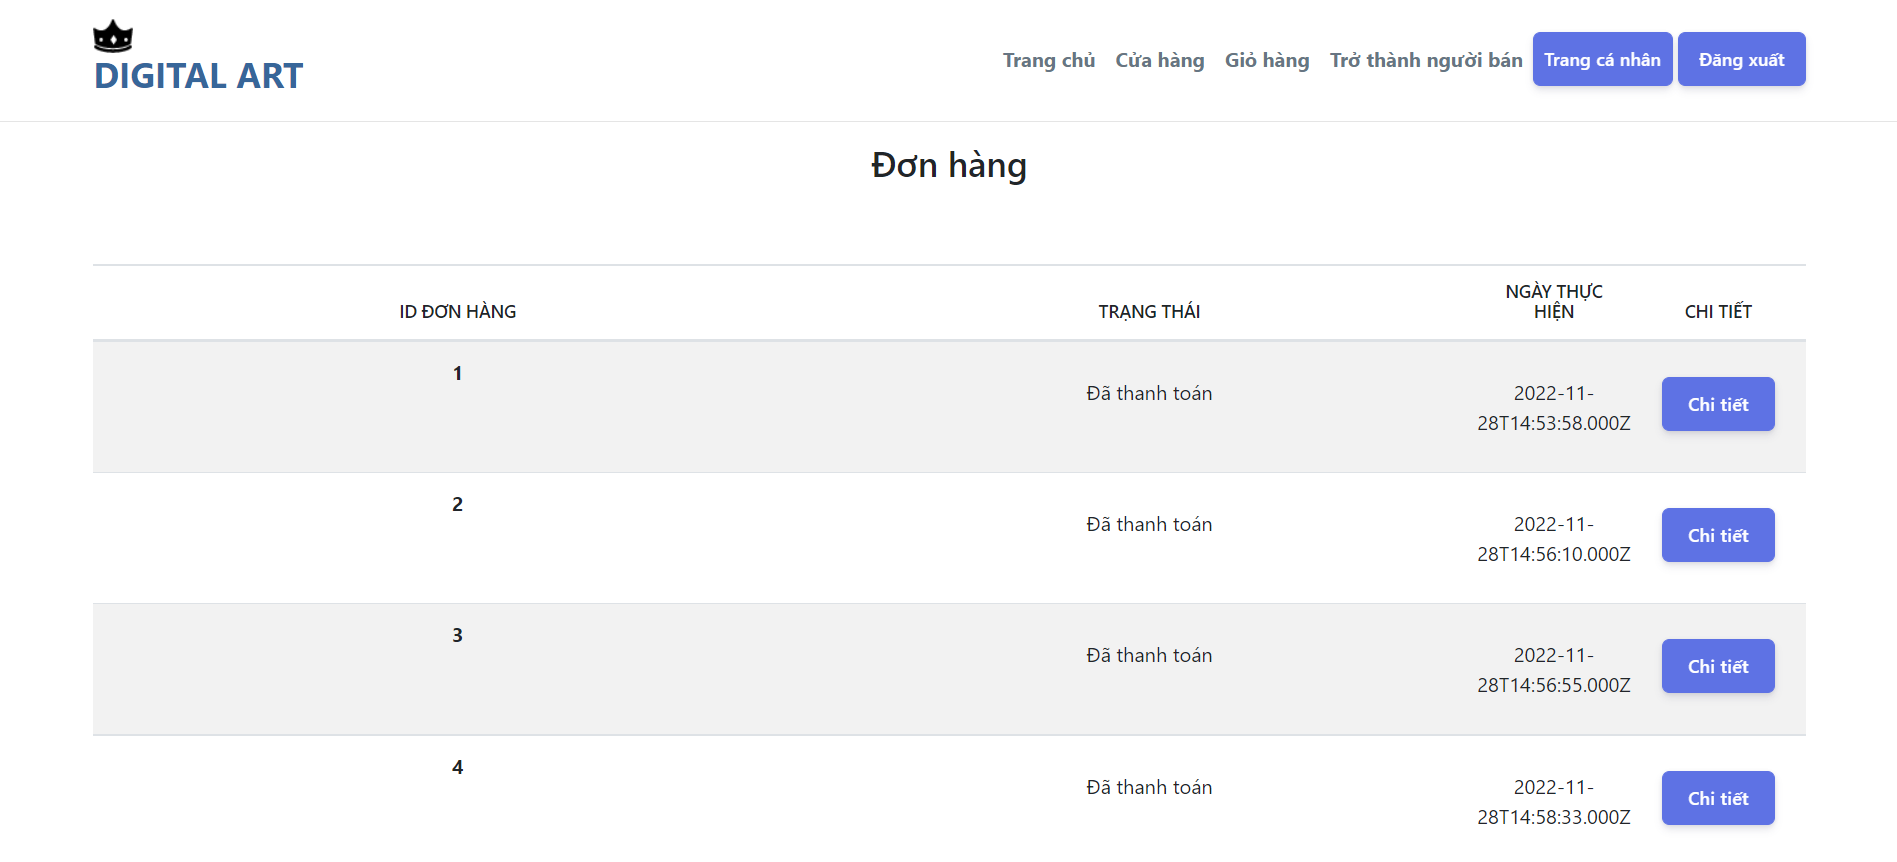
\includegraphics[scale=.400]{anh46.png}
			\end{center}
			\caption{Giao diện thông tin ví điện tử người dùng}
			
		\end{figure}
	\end{center}
}

\newpage
{\large  
	\indent Cửa hàng \\
	{\large
		Người dùng ấn vào phần cửa hàng trên trang chủ hệ thống sẽ chuyển tới trang cửa hàng.}
	\begin{center}
		\begin{figure}[htp]
			\begin{center}
				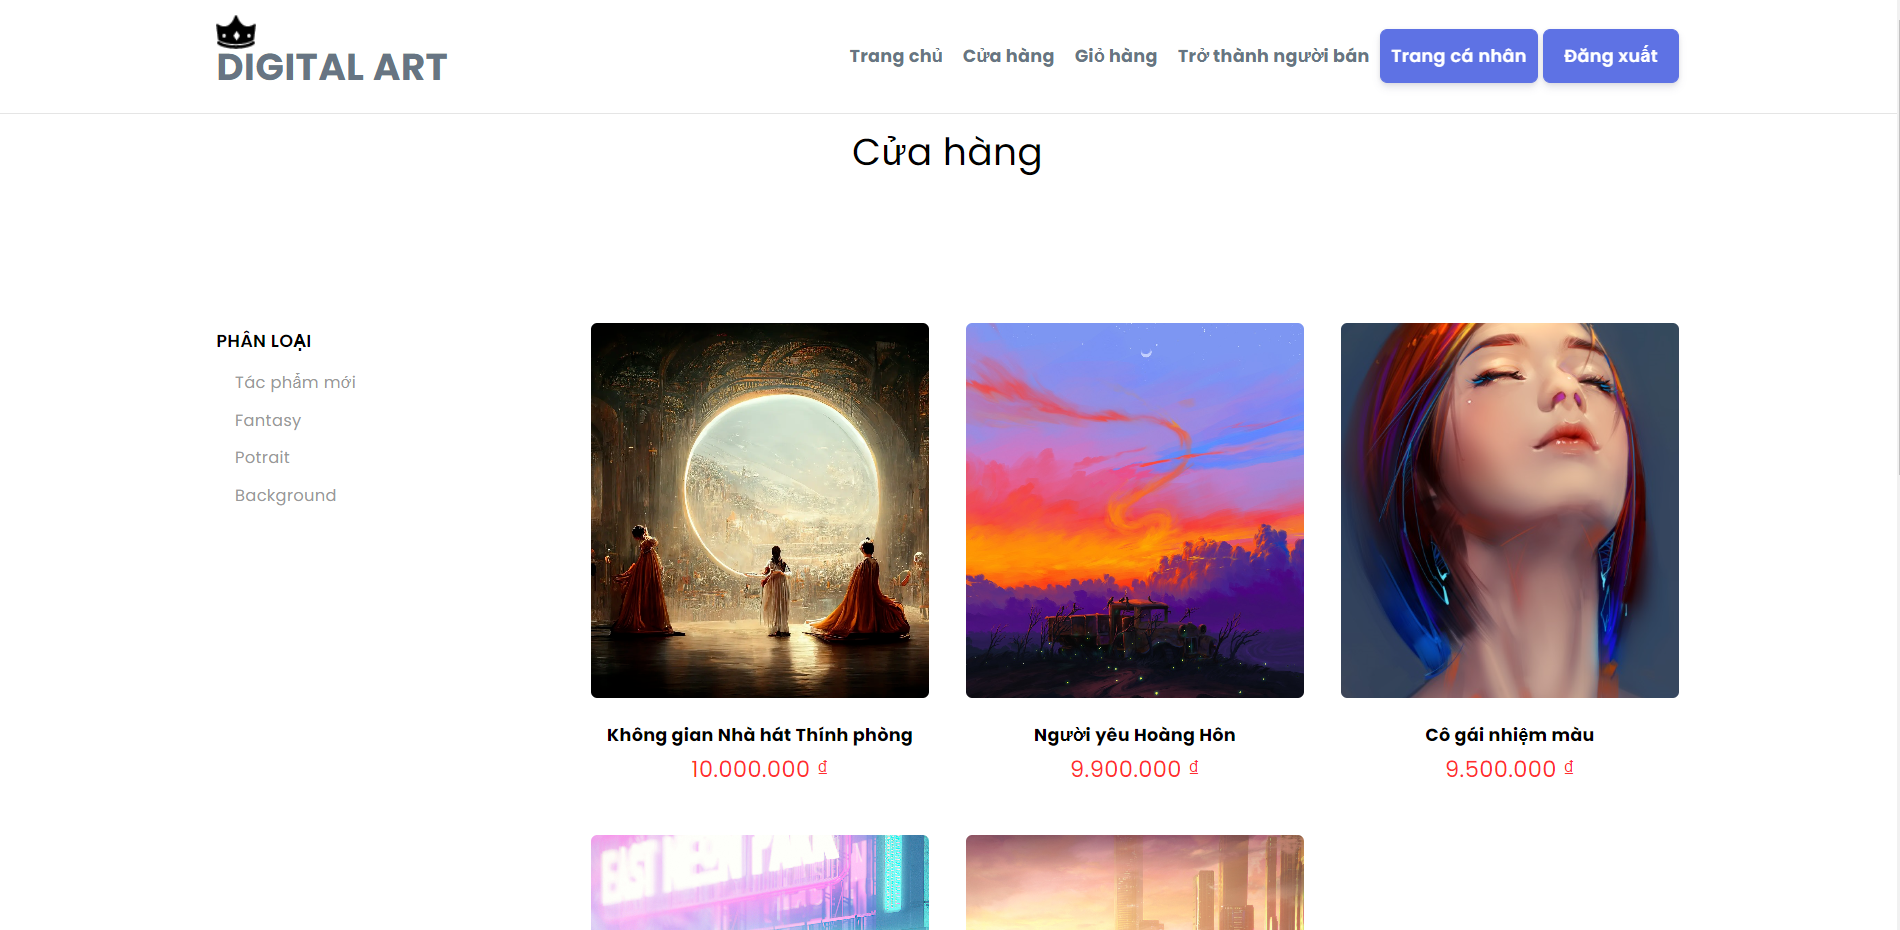
\includegraphics[scale=.400]{anh48.png}
			\end{center}
			\caption{Giao diện cửa hàng}
			
		\end{figure}
	\end{center}
}

\newpage
{\large  
	\indent Trang cá nhân của người dùng \\
	{\large
		Người dùng ấn vào phần trang cá nhân trên trang chủ hệ thống sẽ chuyển tới trang thông tin cá nhân của người dùng.}
	\begin{center}
		\begin{figure}[htp]
			\begin{center}
				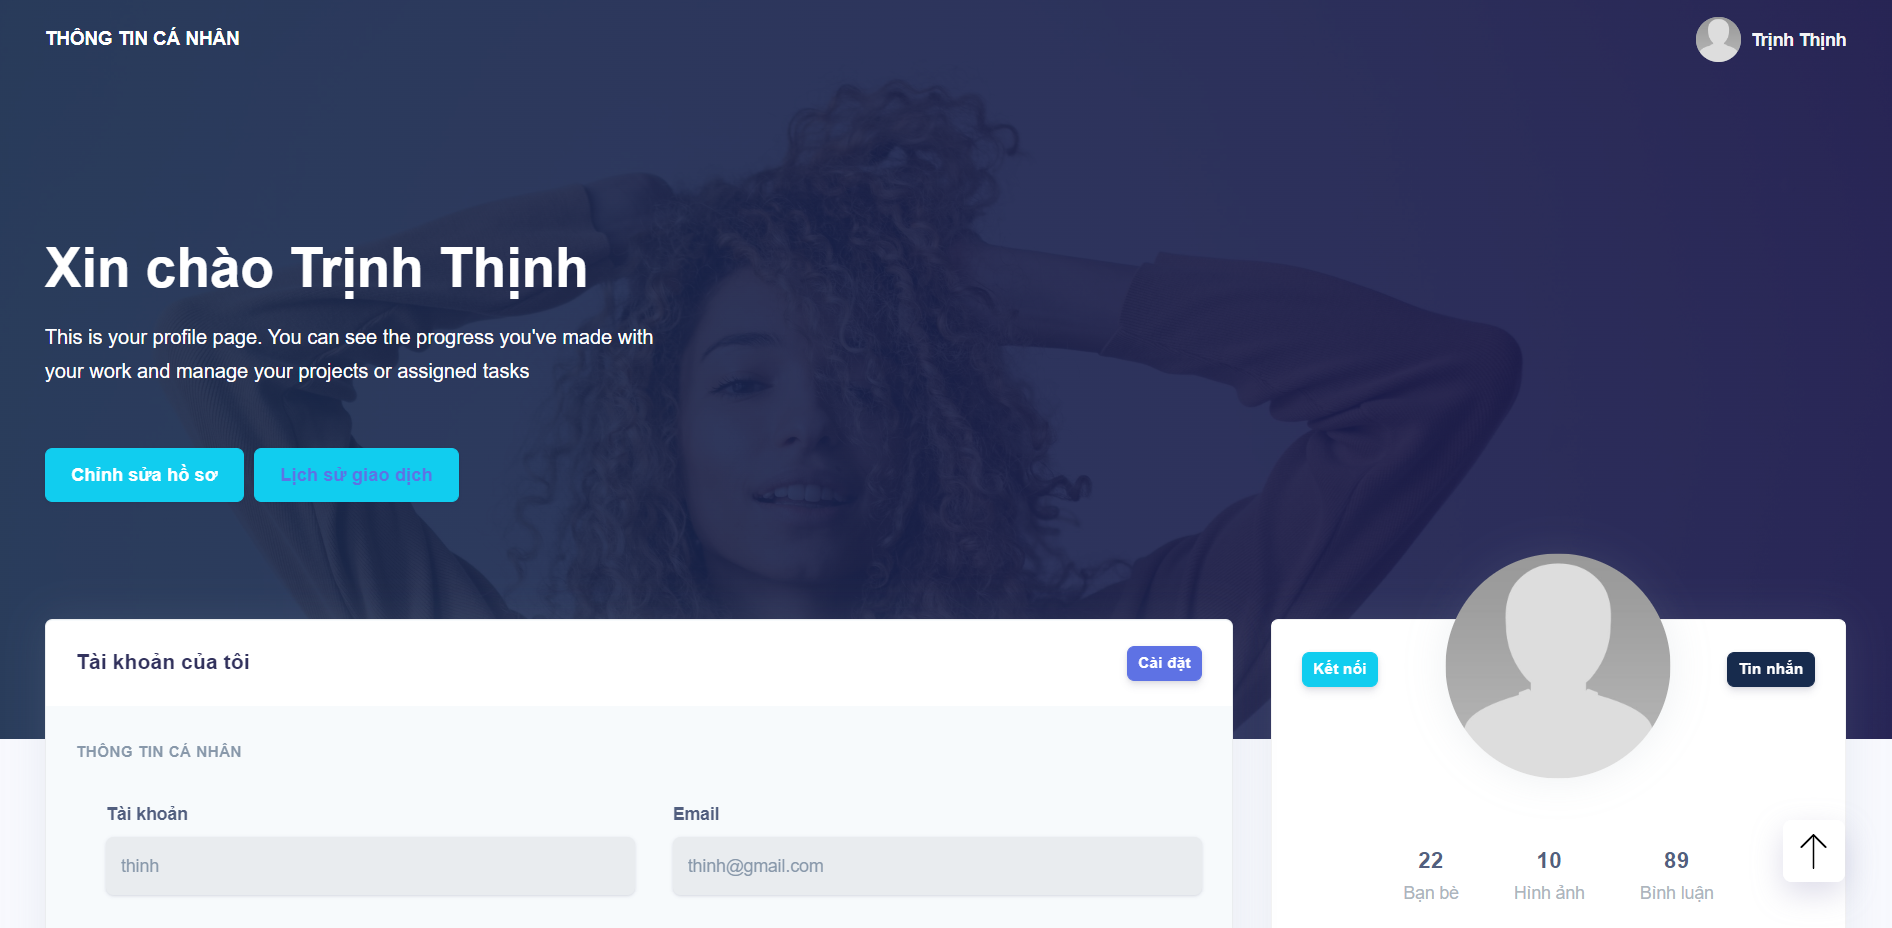
\includegraphics[scale=.400]{anh49.png}
			\end{center}
			\caption{Giao diện trang cá nhân của người dùng}
			
		\end{figure}
	\end{center}
}

\newpage
{\large Các tính năng của Seller\\
	\indent	Quản lý sản phẩm của seller \\
		{\large
		Seller ấn vào phần trang cá nhân trên trang chủ hệ thống sẽ chuyển tới trang thông tin cá nhân sau đó kéo chuột xuống sẽ thấy phần tranh của tôi ở dây seller có thể quản lý tranh của mình.}
	\begin{center}
		\begin{figure}[htp]
			\begin{center}
				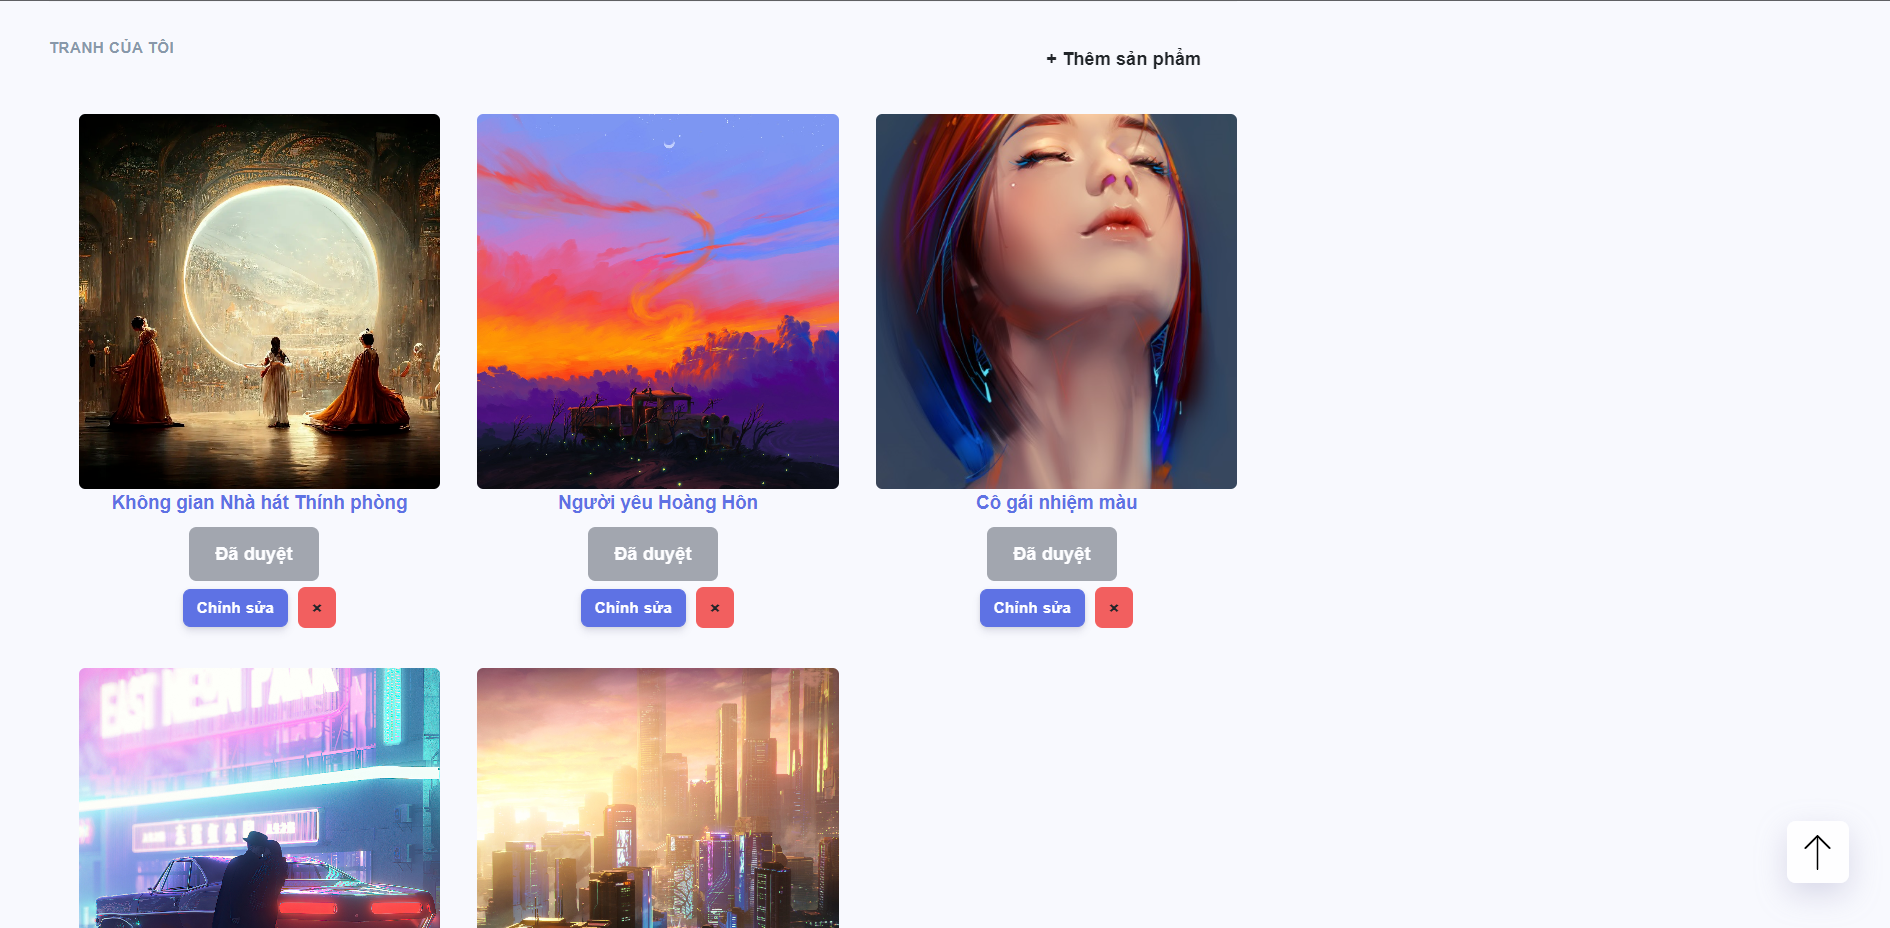
\includegraphics[scale=.400]{anh39.png}
			\end{center}
			\caption{Giao điện quản lý sản phẩm của seller  }
			
		\end{figure}
	\end{center}
}
\newpage
{\large Các tính năng của Admin\\
	\indent Chỉnh sửa thông tin người dùng\\
	{\large
	Admin sau khi đăng nhập bằng tài khoản admin ấn vào phần quản lý người dùng ,sau đó chọn tài tài khoản cần chỉnh sửa thông tin và ấn chỉnh sửa.}
	\begin{center}
		\begin{figure}[htp]
			\begin{center}
				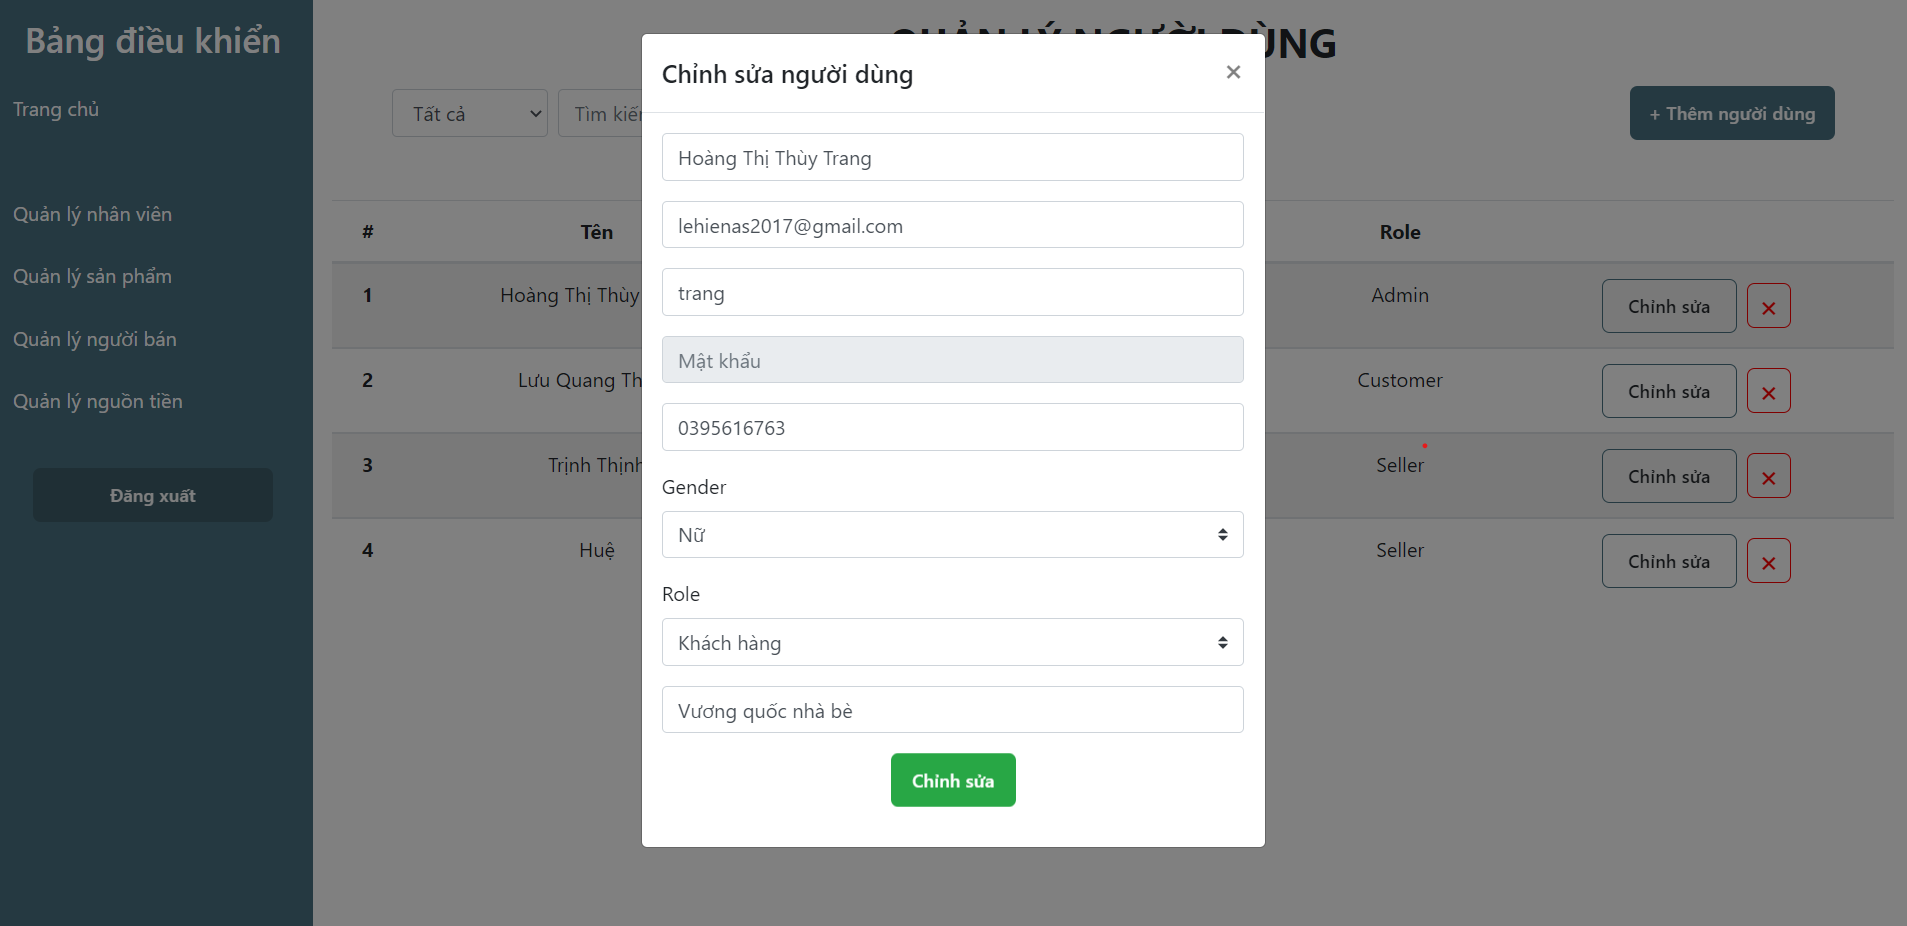
\includegraphics[scale=.400]{anh40.png}
			\end{center}
			\caption{Giao diện chỉnh sửa thông tin người dùng trong admin}
			
		\end{figure}
	\end{center}
}
\newpage
{\large 
	\indent	Thêm người dùng trong admin\\
		{\large
			Admin sau khi đăng nhập bằng tài khoản admin ấn vào phần quản lý người dùng ,sau đó ấn thêm người dùng.}
	\begin{center}
		\begin{figure}[htp]
			\begin{center}
				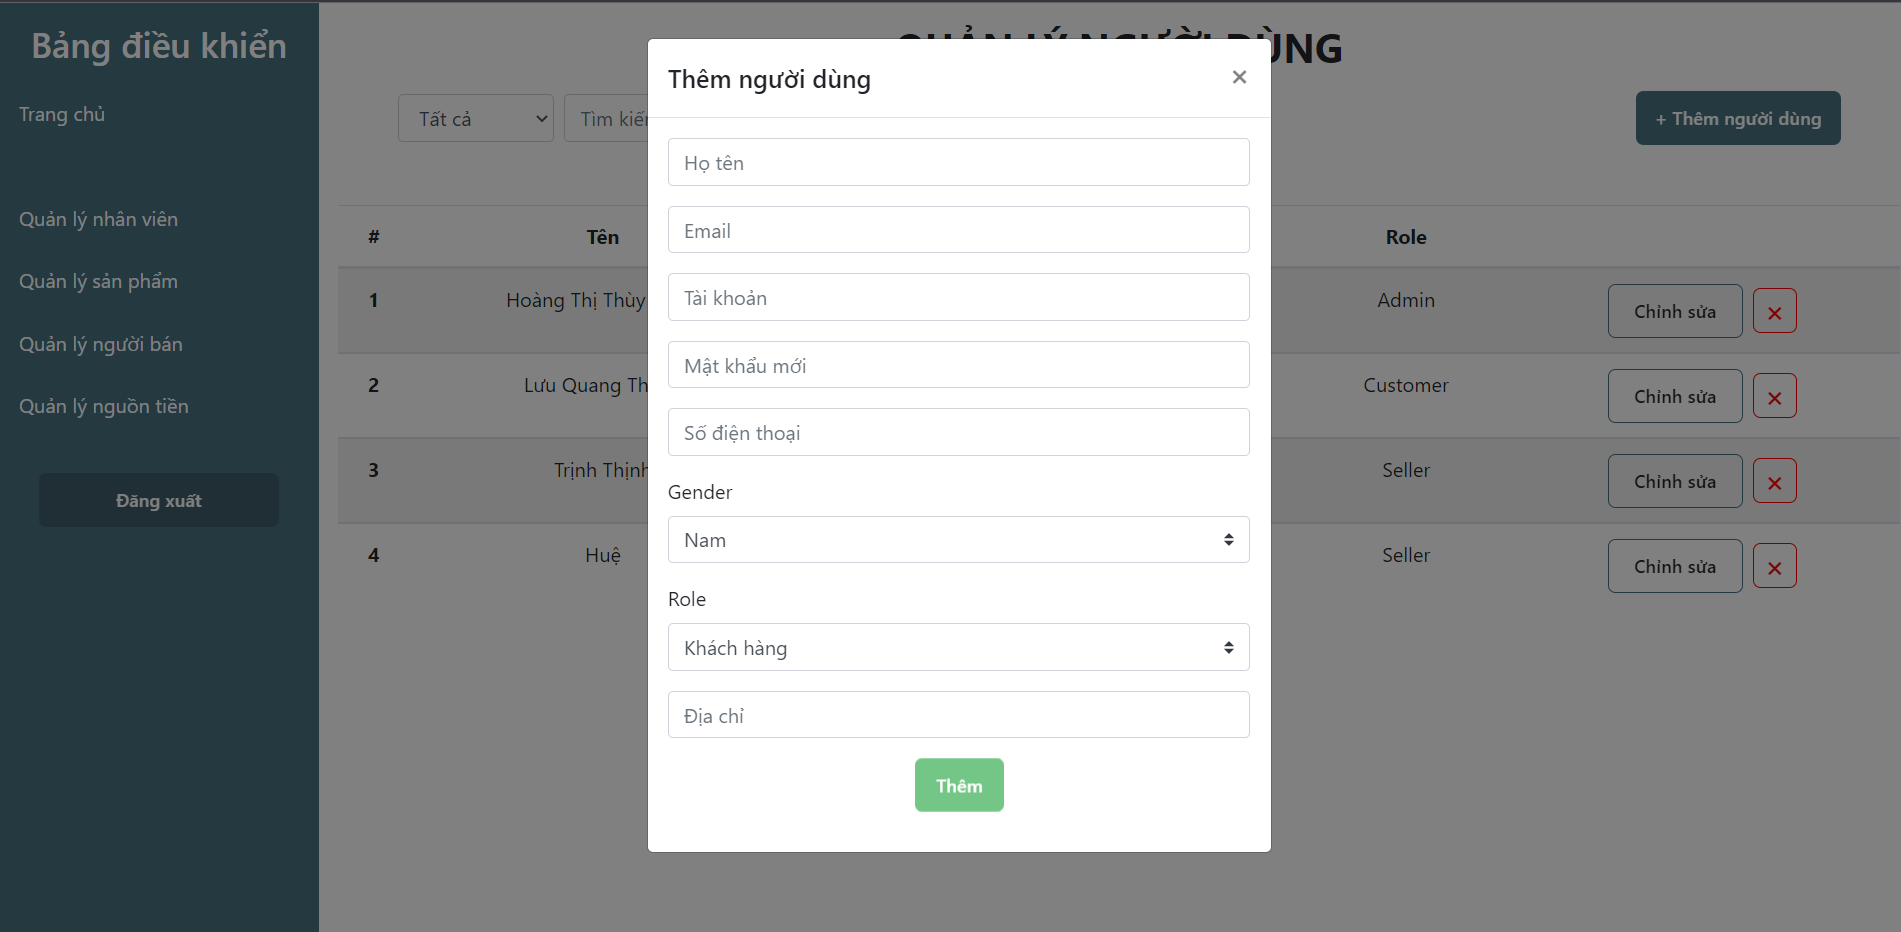
\includegraphics[scale=.400]{anh47.png}
			\end{center}
			\caption{Giao diện thêm người dùng trong admin}
			
		\end{figure}
	\end{center}
}
\newpage

{\large  
	\indent Quản lý thông tin người dùng\\
		{\large
	Admin sau khi đăng nhập bằng tài khoản admin ấn vào phần quản lý người dùng ở đây sẽ hiển thị danh sách tài khoản người dùng.}
	\begin{center}
		\begin{figure}[htp]
			\begin{center}
				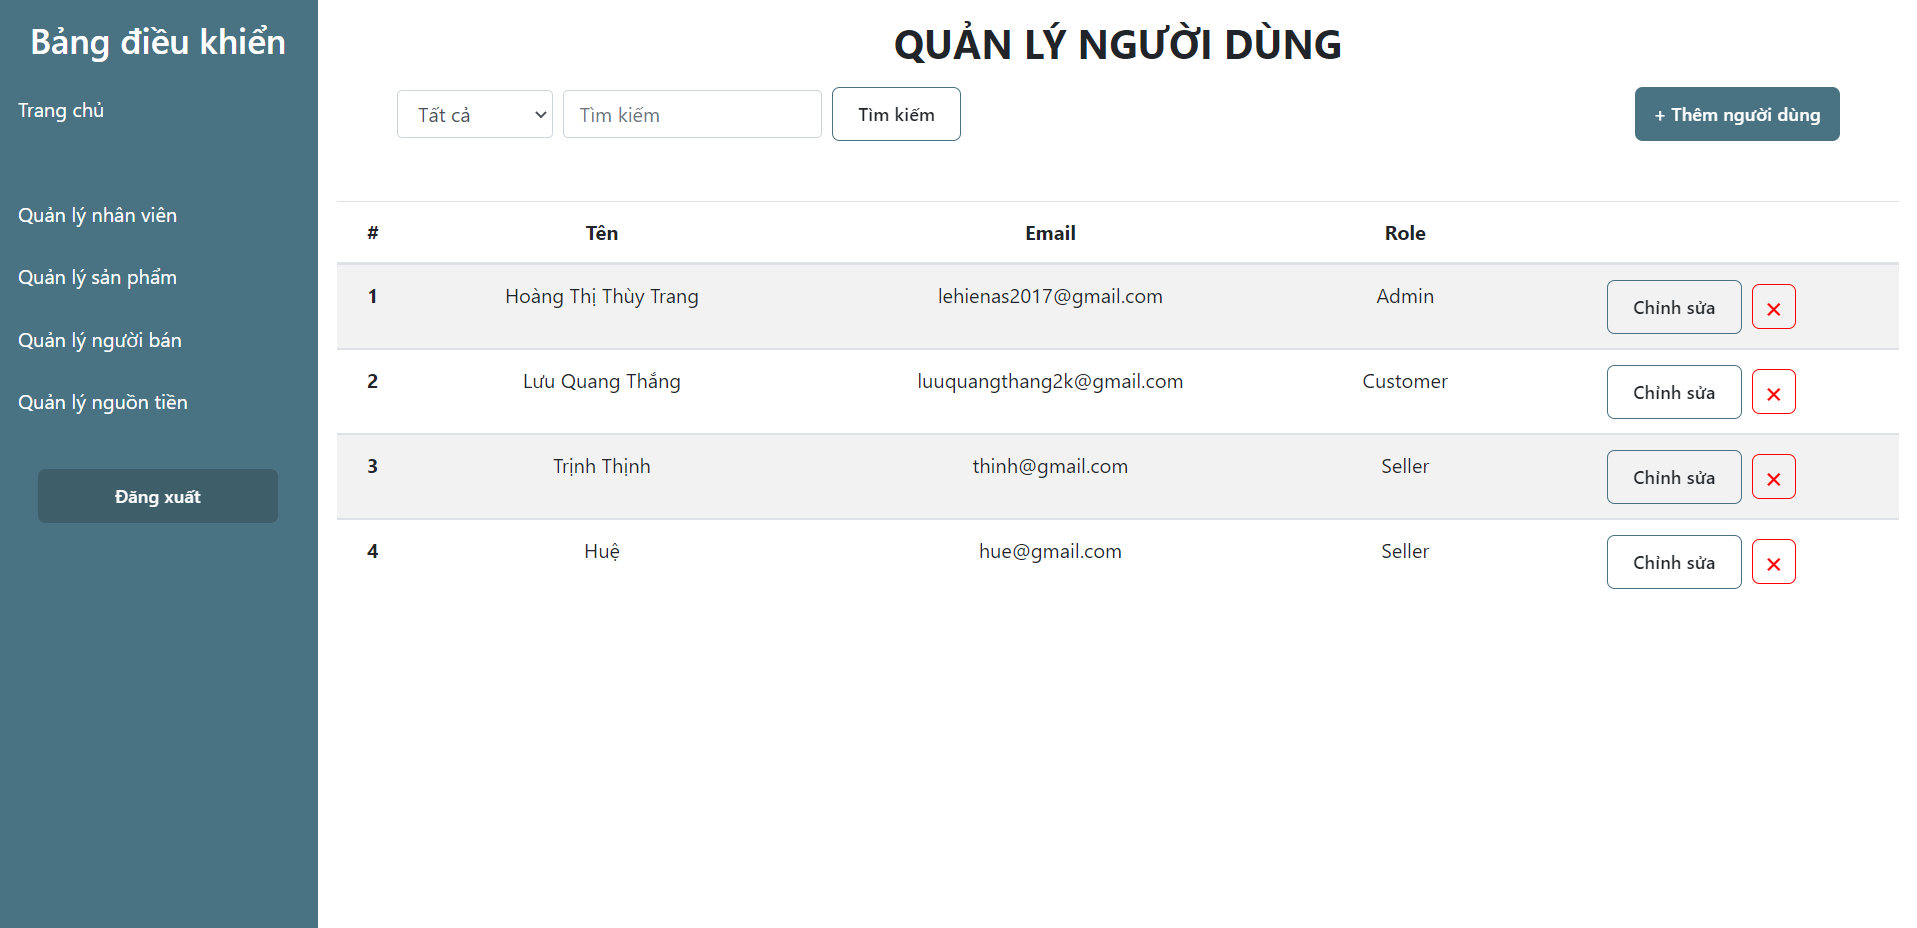
\includegraphics[scale=.400]{anh41.png}
			\end{center}
			\caption{Giao diện quản lý thông tin người dùng}
			
		\end{figure}
	\end{center}
}
\newpage
{\large  
	\indent Duyệt thông tin đăng ký làm seller\\
		{\large
		Sau khi đăng nhập bằng tài khoản admin ấn vô phần quản lý người bán  ở đây admin có thể duyệt các đơn trở thành seller của người dùng.}
	\begin{center}
		\begin{figure}[htp]
			\begin{center}
				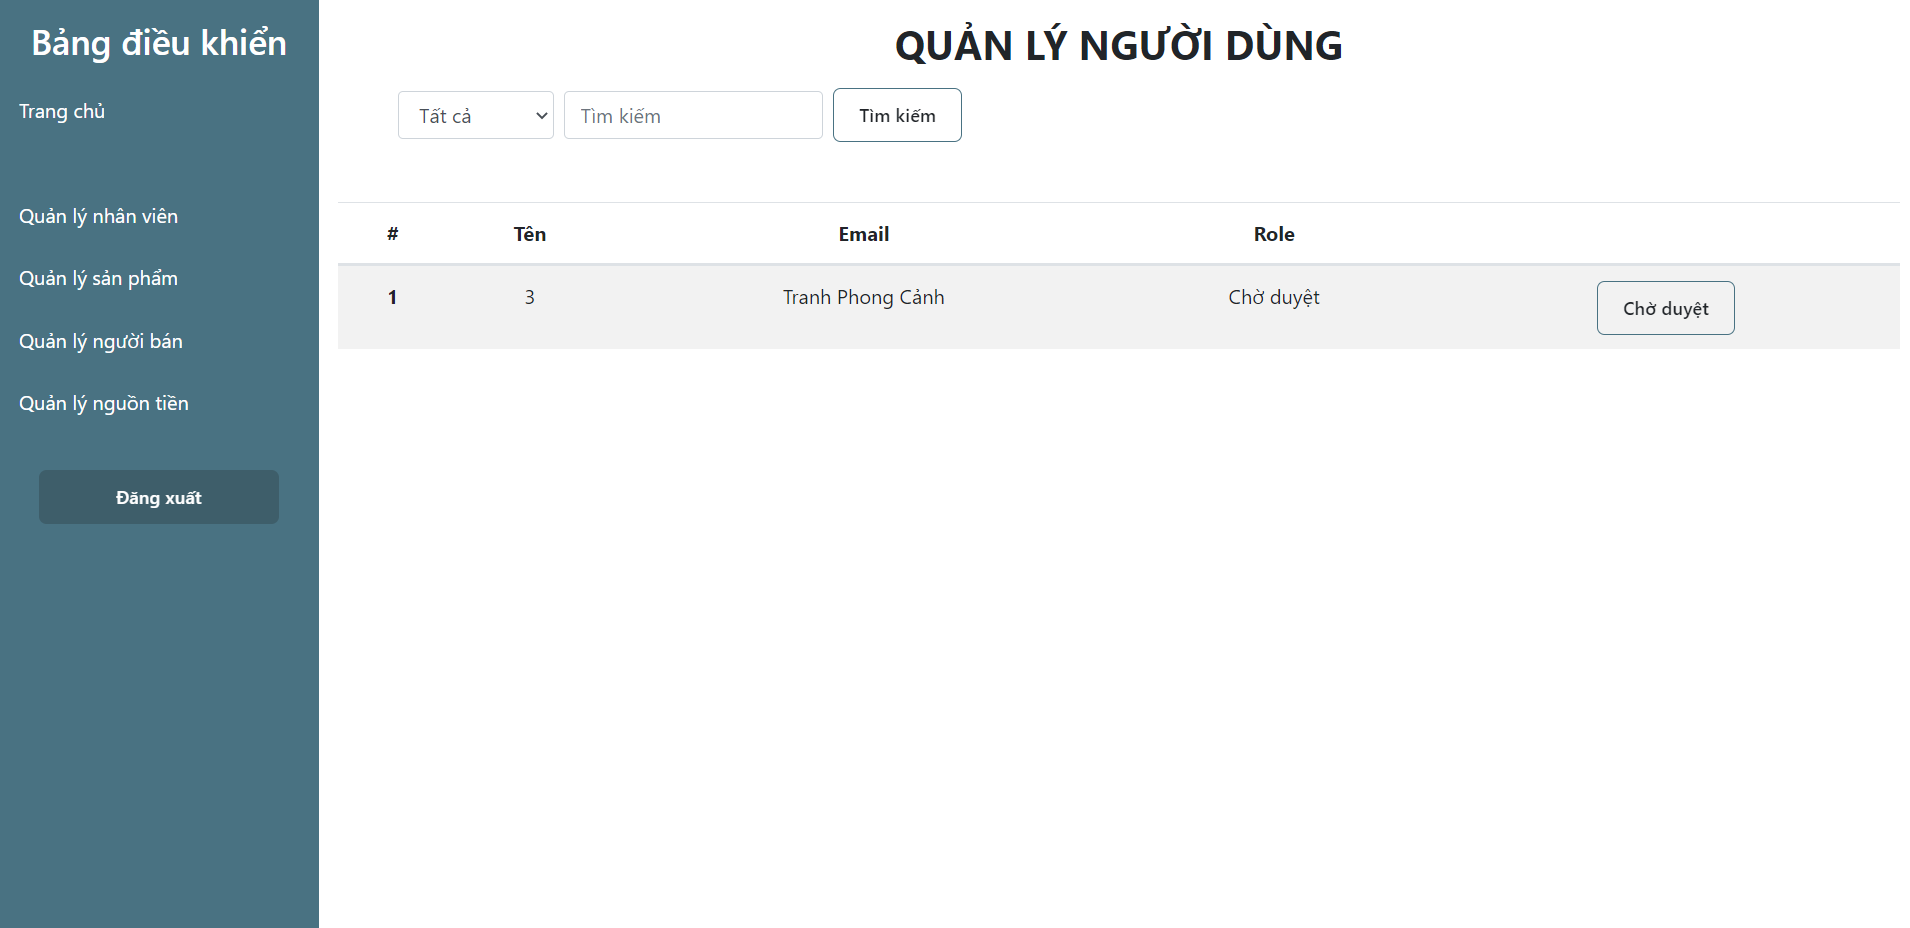
\includegraphics[scale=.400]{anh42.png}
			\end{center}
			\caption{Giao diện duyệt thông tin đăng ký làm seller}
			
		\end{figure}
	\end{center}
}
\newpage
{\large  
	\indent Chỉnh sửa thông tin sản phẩm khi duyệt\\
	{\large
		Sau khi đăng nhập bằng tài khoản admin ấn vô phần quản lý sản phẩm  ở đây admin có thể thấy chọn sản phẩm cần sửa thông tin trước khi duyệt và ấn chỉnh sửa.}
	\begin{center}
		\begin{figure}[htp]
			\begin{center}
				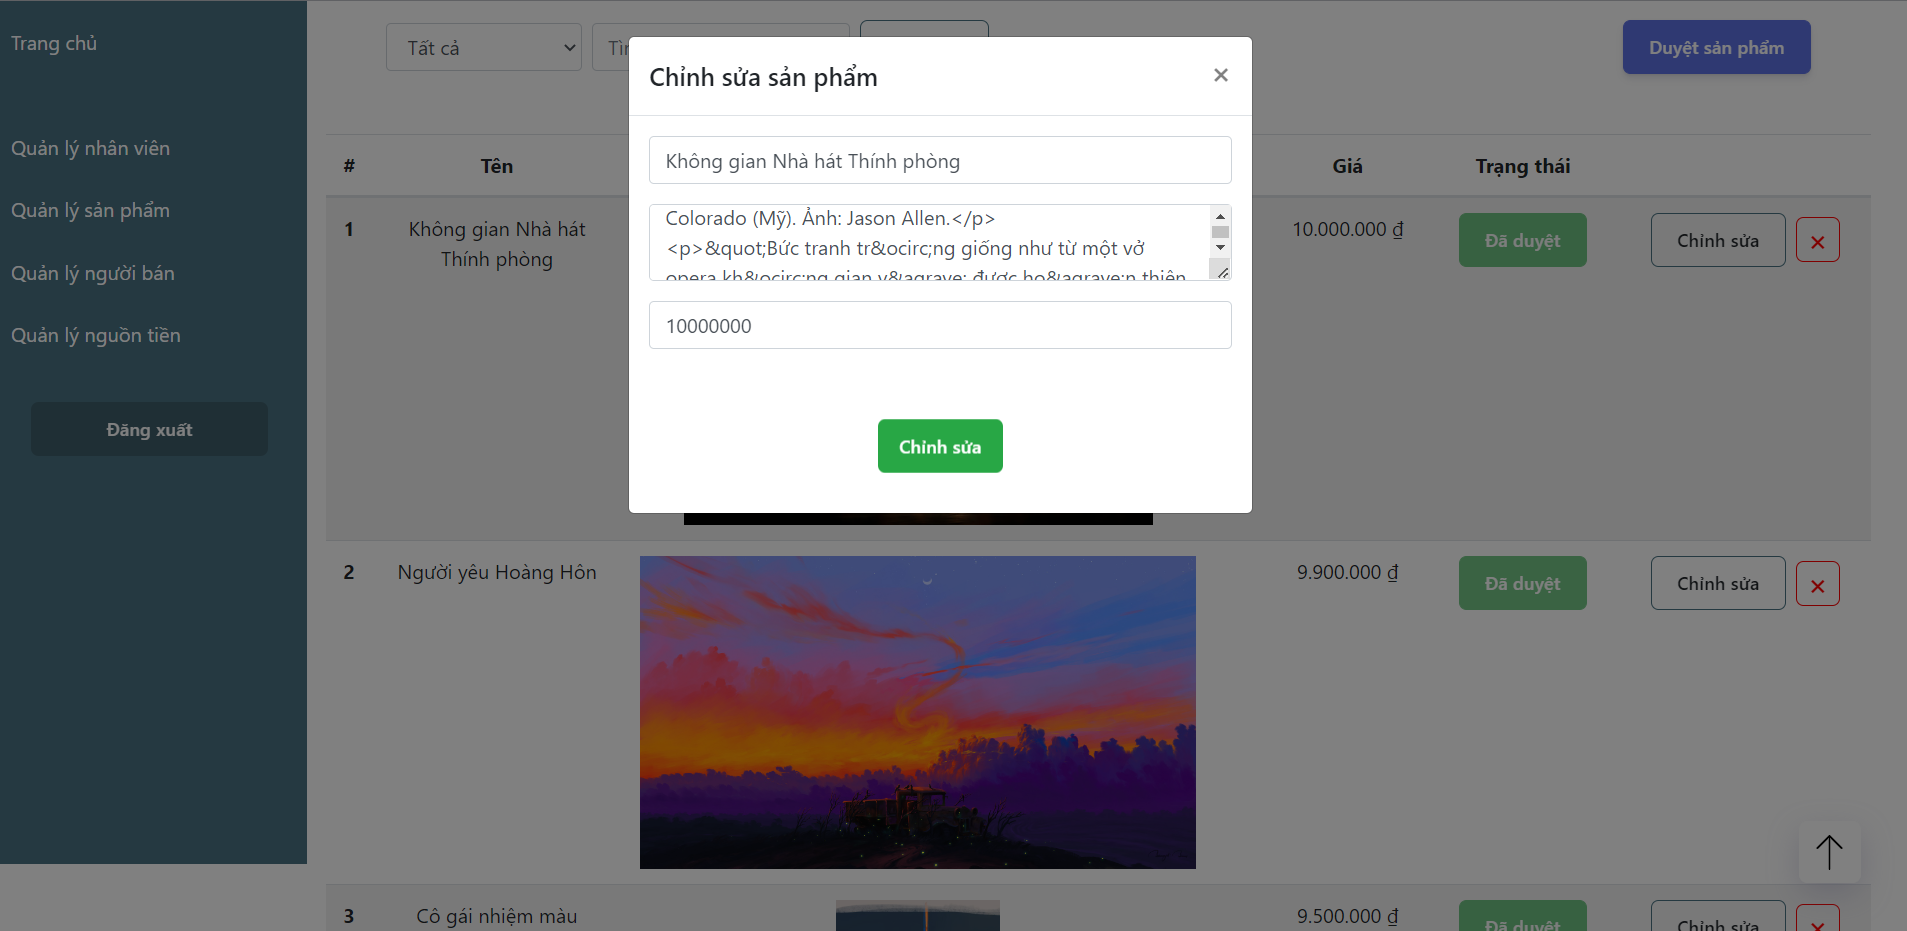
\includegraphics[scale=.400]{anh43.png}
			\end{center}
			\caption{Giao diện chỉnh sửa thông tin sản phẩm khi duyệt}
			
		\end{figure}
	\end{center}
}

\newpage
{\large  
	\indent Quản lý sản phẩm cần duyệt\\
	{\large
		Sau khi đăng nhập bằng tài khoản admin ấn vô phần quản lý sản phẩm ở đây admin có thể thấy danh sách các sản phẩm cần duyệt trước khi bán.}
	\begin{center}
		\begin{figure}[htp]
			\begin{center}
				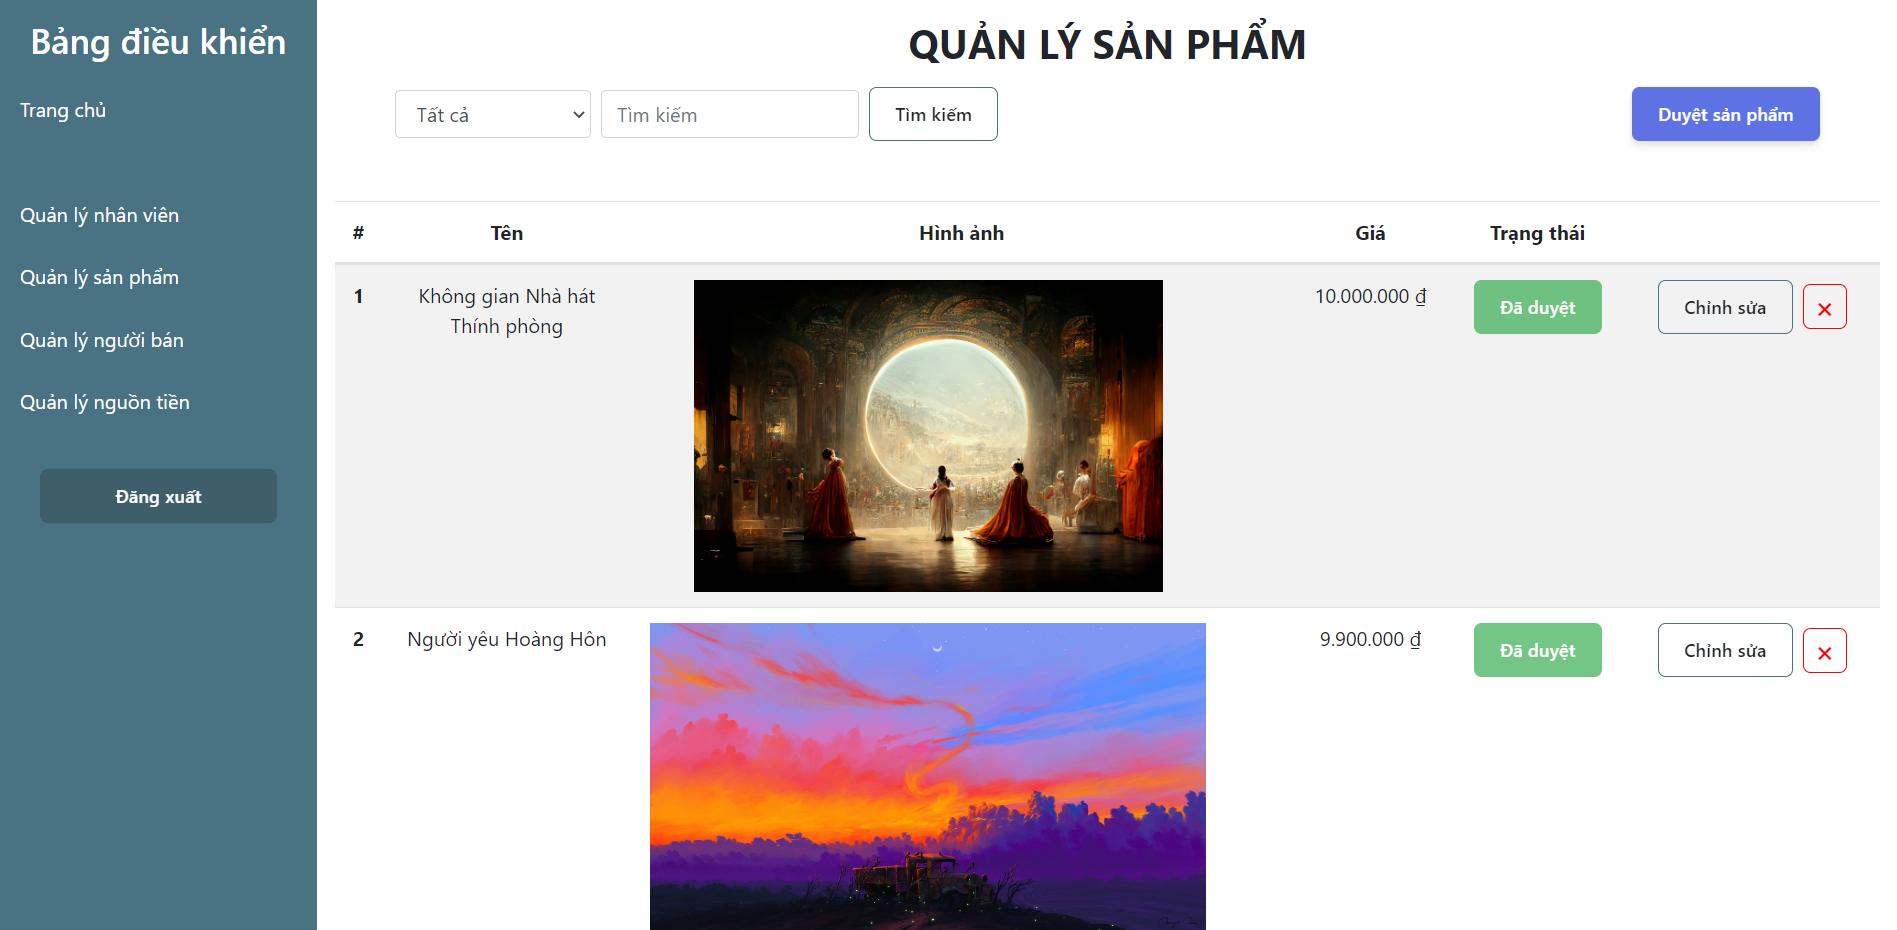
\includegraphics[scale=.400]{anh44.png}
			\end{center}
			\caption{Giao diện quản lý thông tin sản phẩm cần duyệt}
			
		\end{figure}
	\end{center}
}

\newpage
{\large  
	\indent Quản lý nguồn tiền\\
		{\large
		Sau khi đăng nhập bằng tài khoản admin ấn vô phần quản lý nguồn tiền  ở đây admin có thể thấy thông tin ví admin như lịch sử giao dịch số dư}
	\begin{center}
		\begin{figure}[htp]
			\begin{center}
				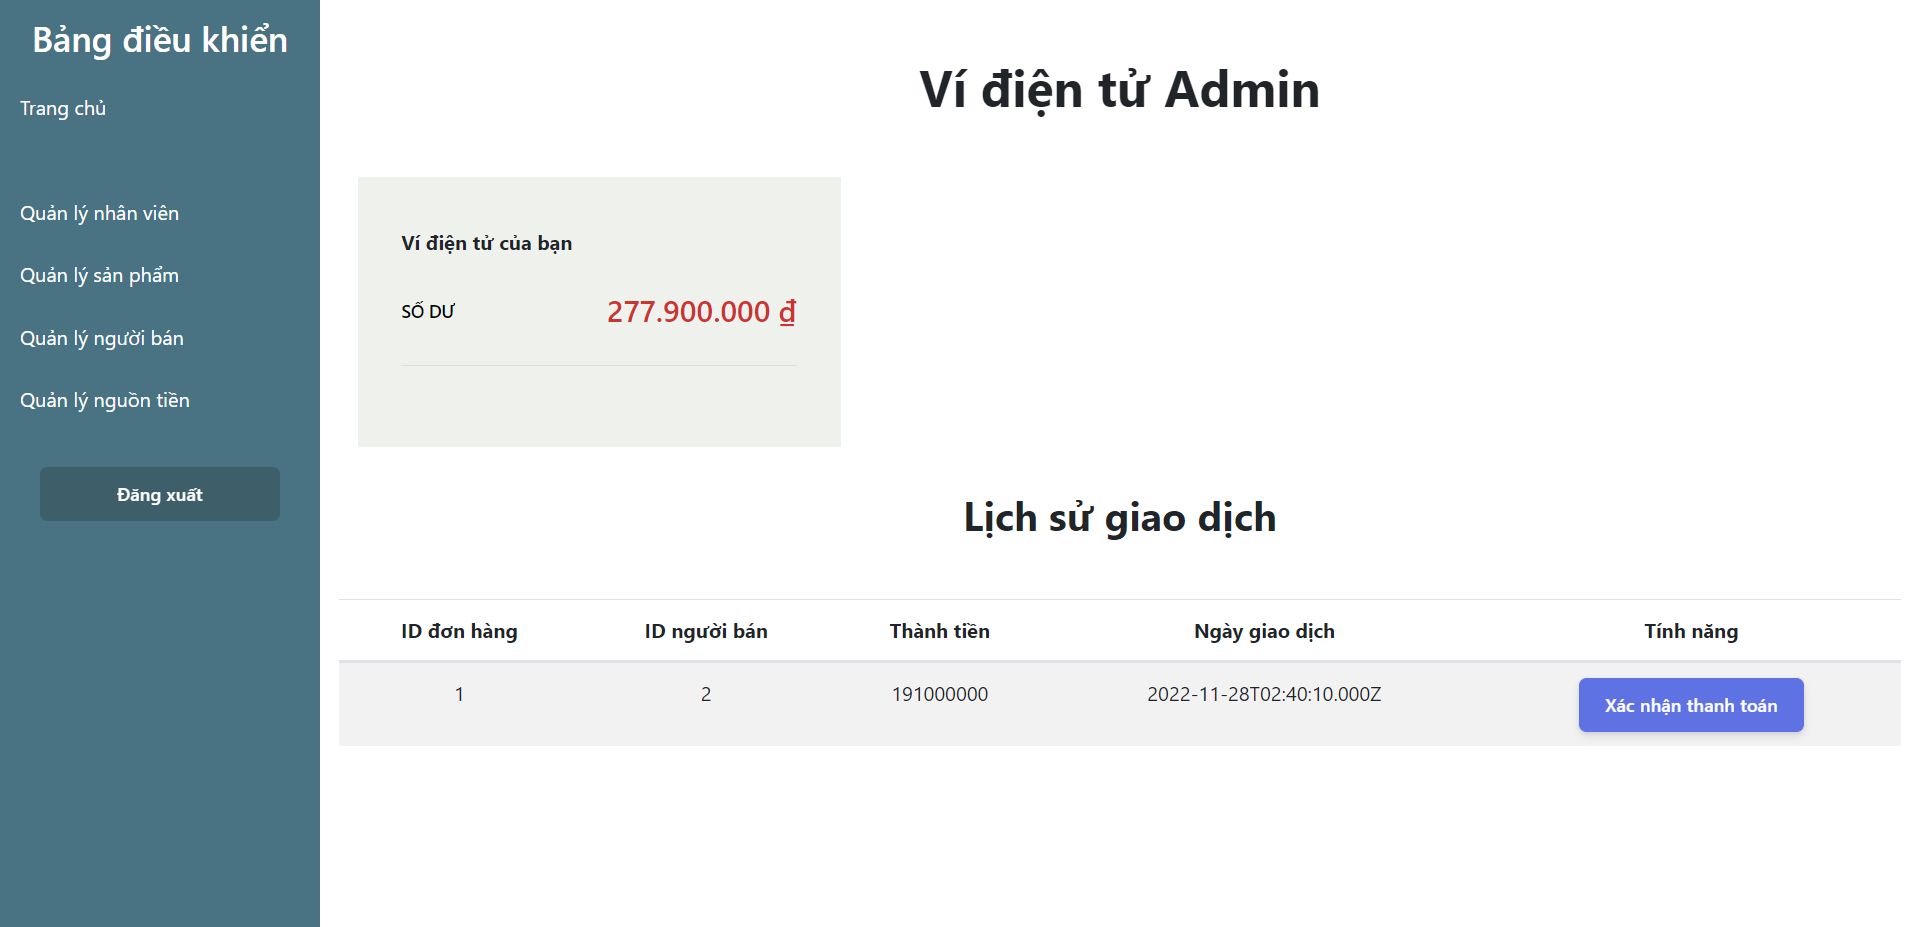
\includegraphics[scale=.400]{anh45.png}
			\end{center}
			\caption{Giao diện quản lý nguồn tiền}
			
		\end{figure}
	\end{center}
}

\newpage

\section{KẾT LUẬN}
\label{sec:kết luận}
\subsection{Tổng kết}
{
	\large Nhóm chúng em đã tạo được hệ thống bán tranh digital cung cấp được nơi kết nối những nhà sáng tạo nghệ thuật với người yêu thích nghệ thuật ,họ có thể trao đổi mua bán tác phẩm một cách nhanh chóng và tiện lợi\\
}
\subsection{Định hướng phát triển trong tương lai}
{
	\large - Nhóm chúng em sẽ tiếp tục khắc phục những điểm yếu của hệ thống. \\
\indent	-Bổ sung thêm các tính năng nâng cao hơn như gợi ý tranh theo sở thích mỗi cá nhân, cho phép nhiều hình thức thanh toán hơn.
	
	
}\newpage

\section{TÀI LIỆU THAM THẢO}
	{
		\large \noindent   -https://niithanoi.edu.vn/nodejs-la-gi-tong-hop-day-du-ve-nodejs-ban-can-biet.html\\
		- https://viblo.asia/p/gioi-thieu-ve-reactjs-phan-i-cac-khai-niem-co-ban-V3m5WzjblO7\\
		
		
	}
\end{document}